\chapter*{Appendix}
%%%%%%%%%%%%%%%%%%%%%%%%%%%%%%%%%%
% ------ Common report --------- %

\section{Documents from Usability Test}
\label{app:usability_documents}
% ------ invitation to usability test --------- %
	\begin{figure}[H]
		\begin{center}
			
\includegraphics[width=\textwidth]{Appendix/invitation_to_usability_test.pdf}
		\end{center}
		\caption{Invitation sent to the test persons of the usability test.}
		\label{appendice:usability_test}
	\end{figure}
	
	\begin{figure}[H]
		\begin{center}
			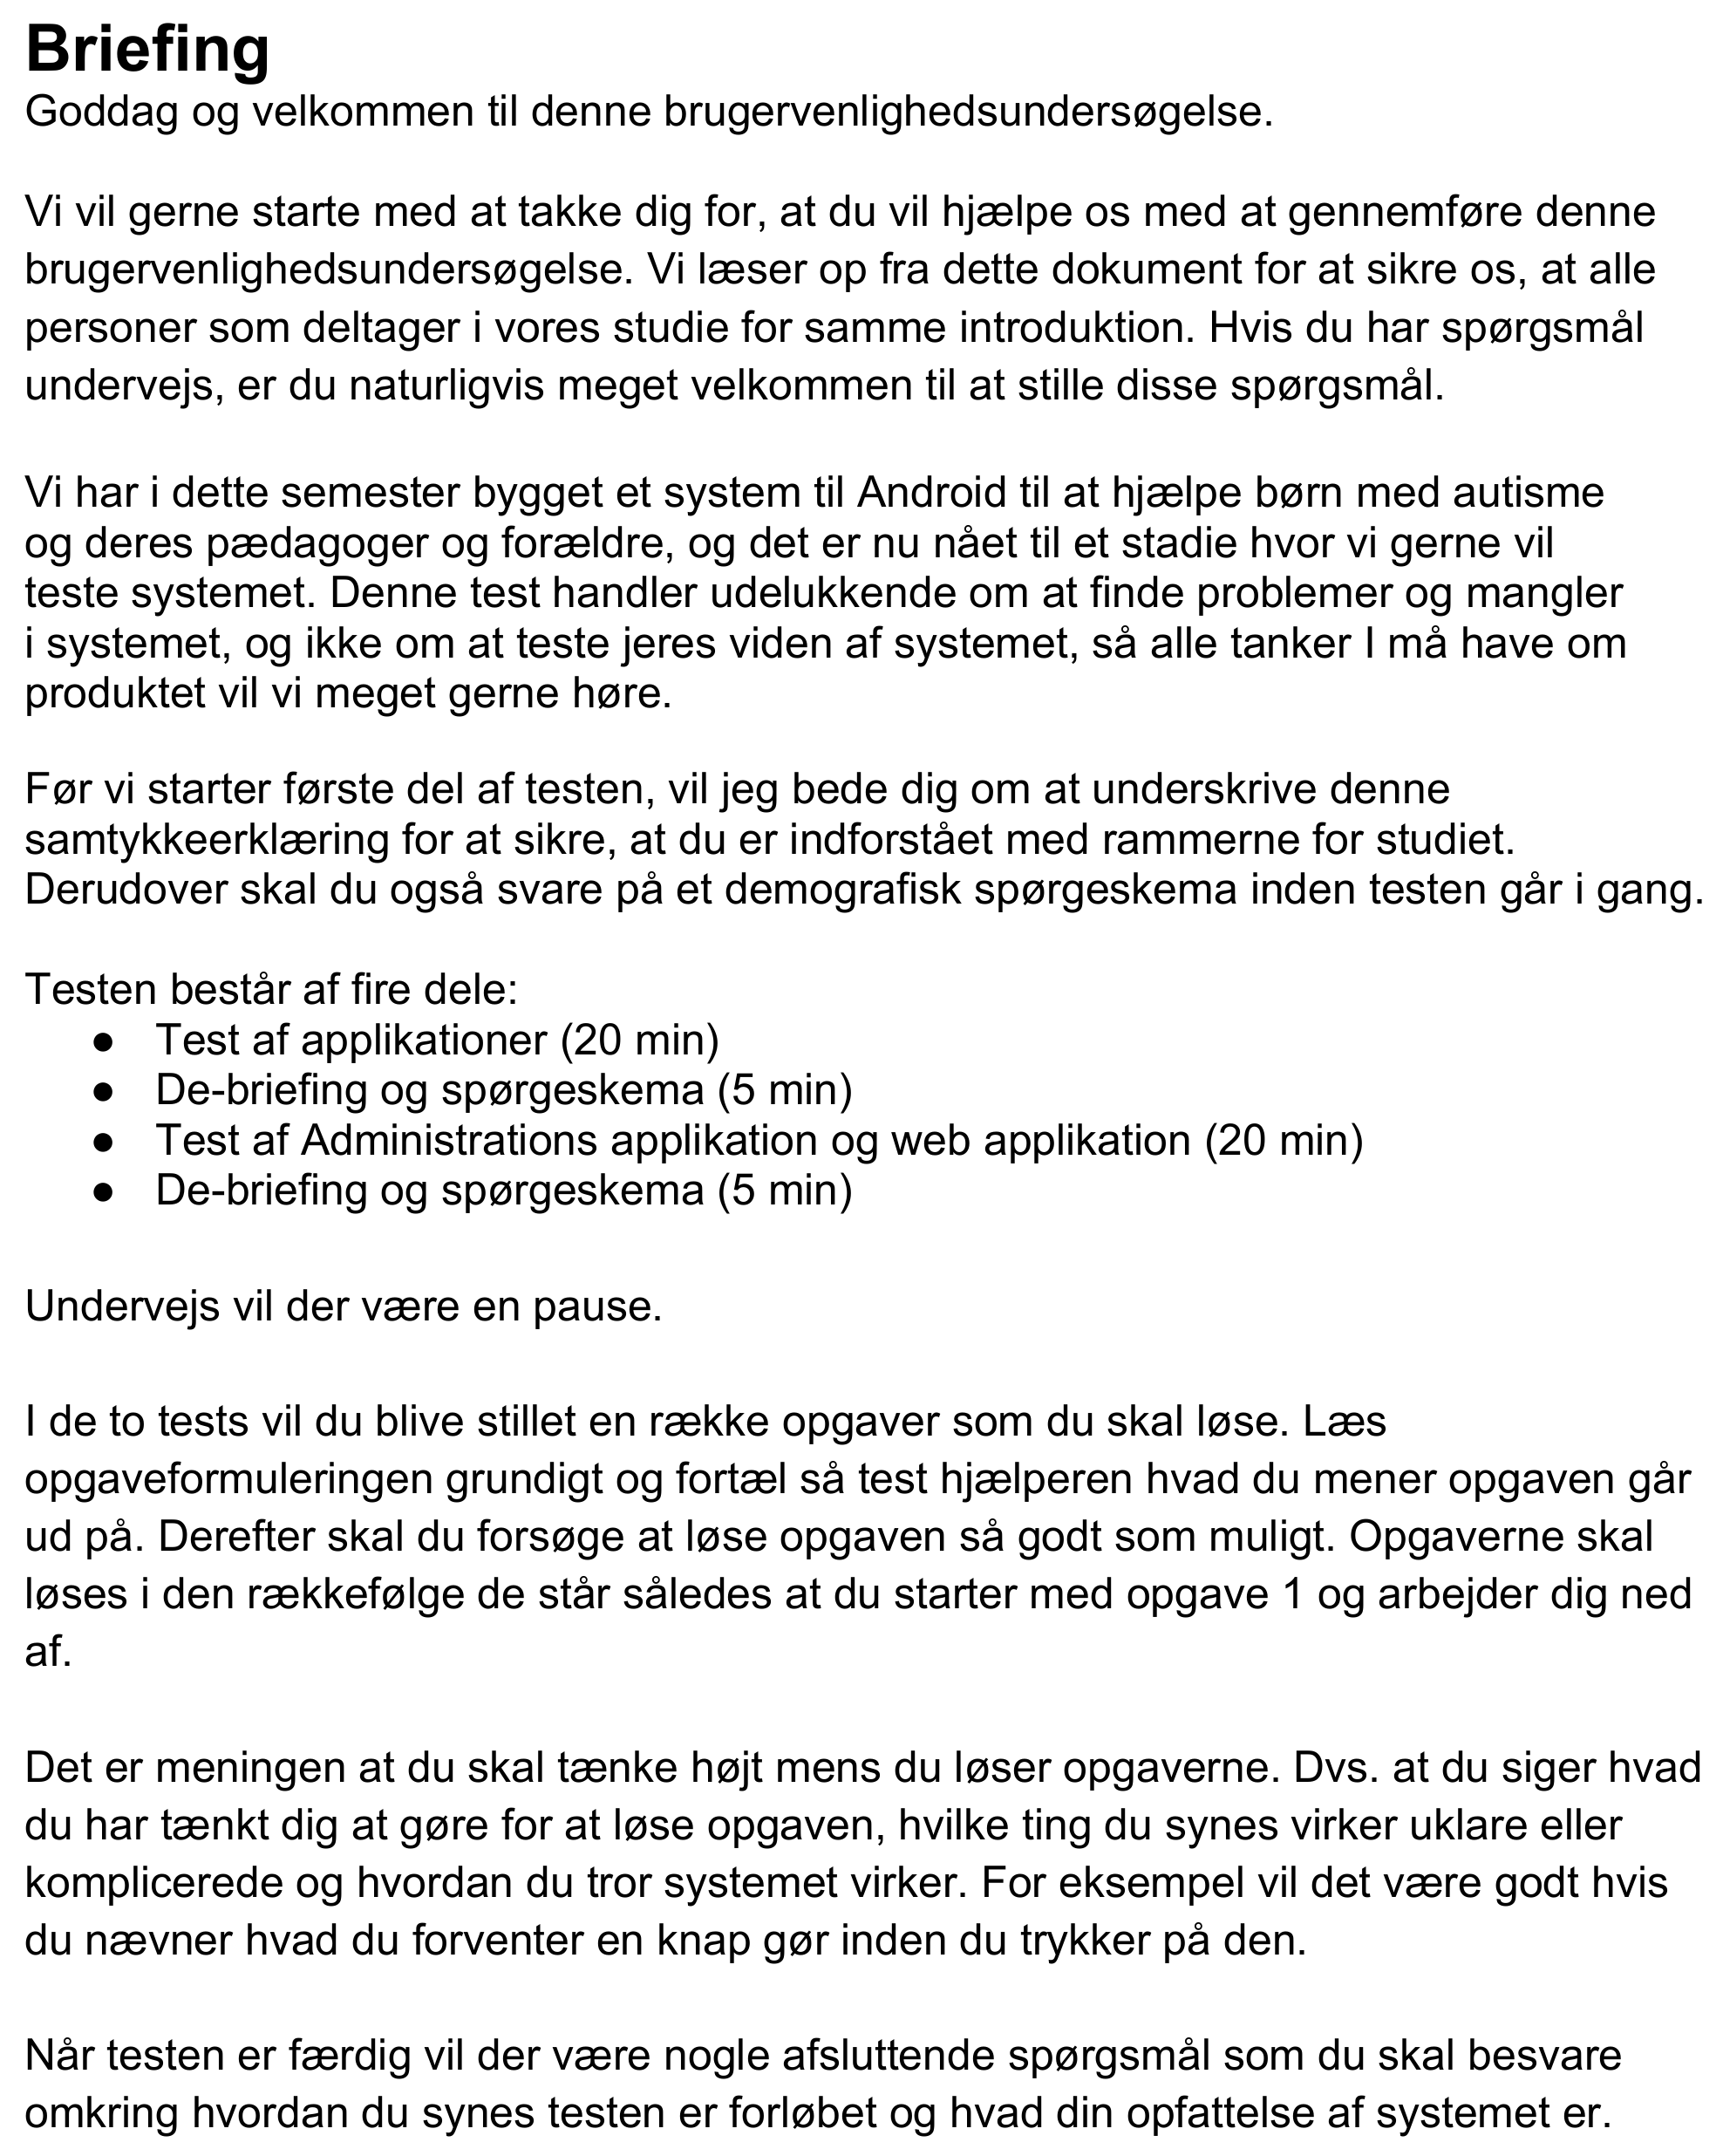
\includegraphics[width=\textwidth]{Appendix/usability-briefing.png}
		\end{center}
		\caption{Briefing which is read aloud to the test persons.}
		\label{appendice:usability_briefing}
	\end{figure}
	
% ------ Questionnaires ------- %
\subsection{Questionnaires from usability}

\label{questionnaires}

\begin{figure}[h]
	\centering
		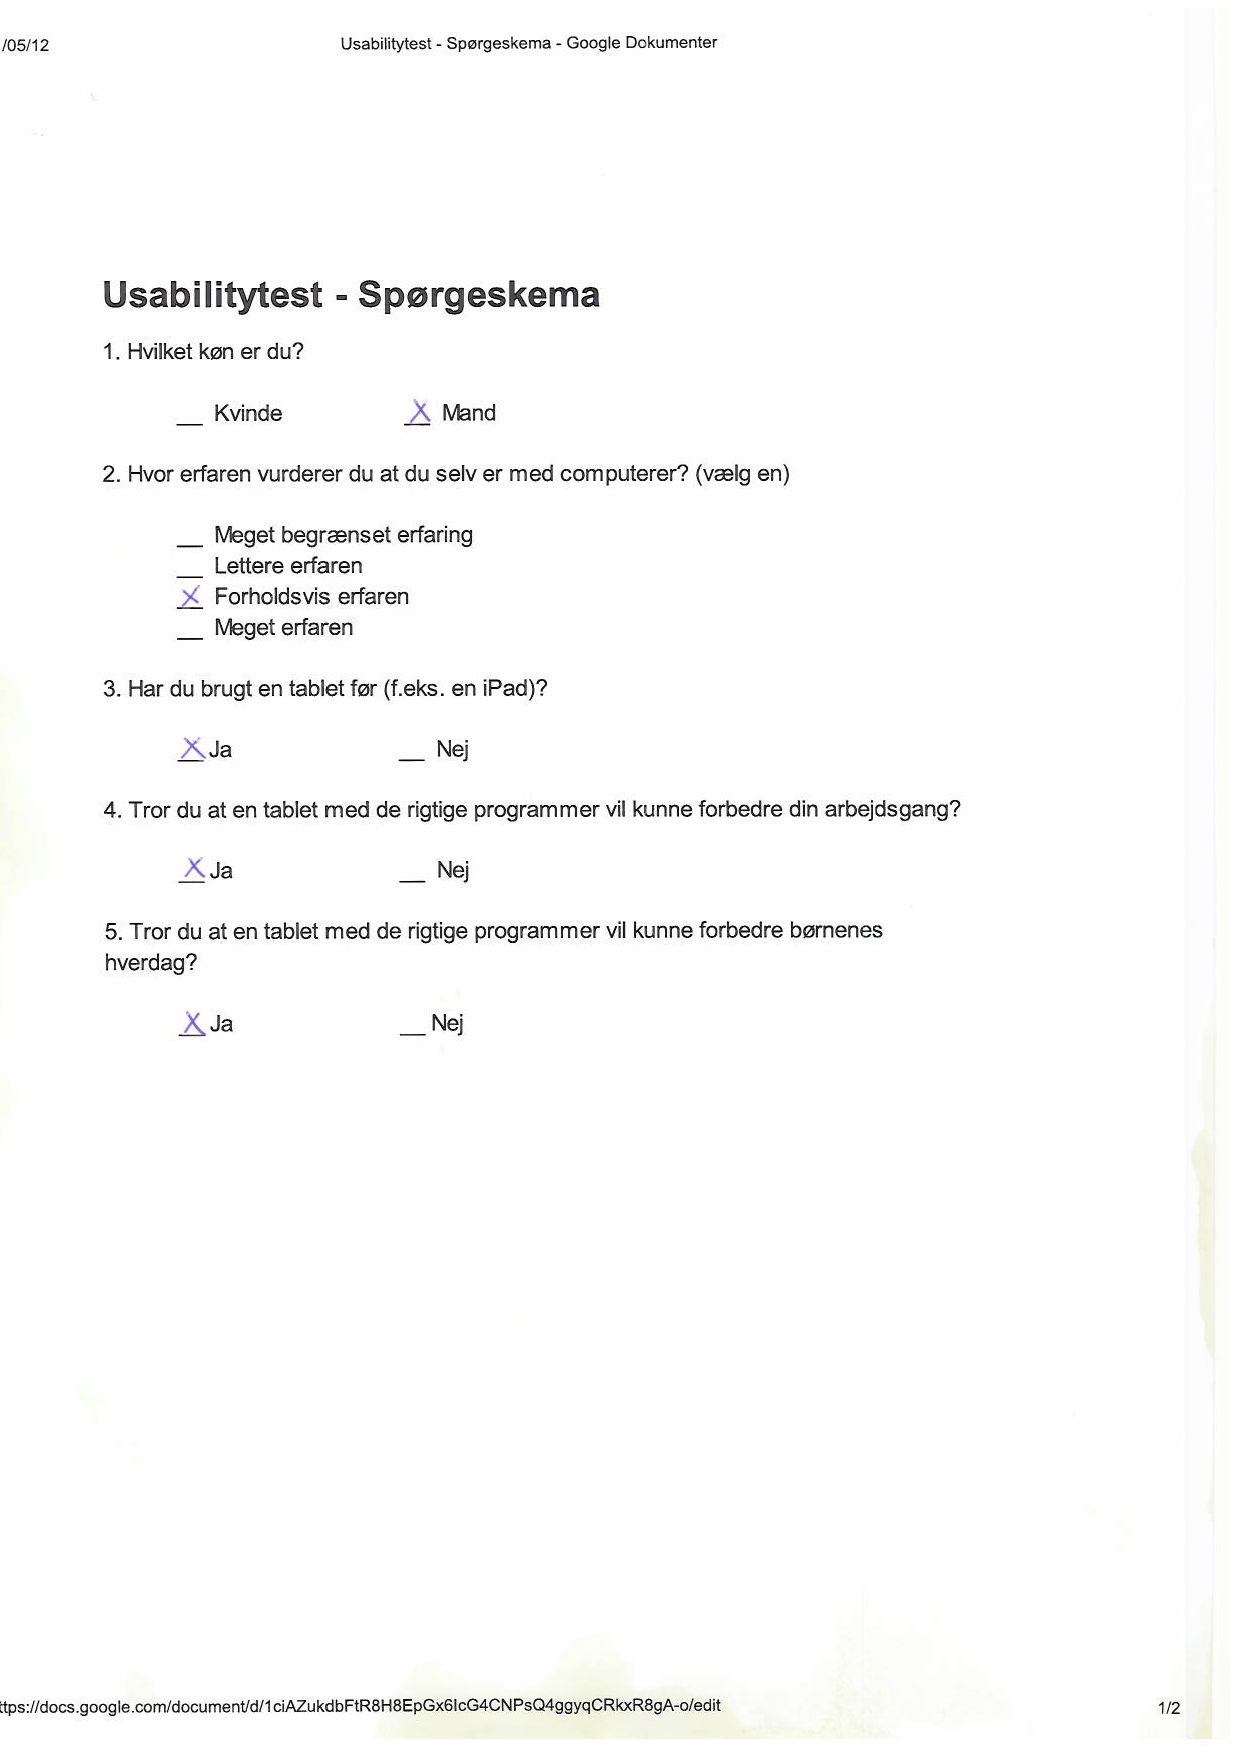
\includegraphics{Appendix/demo_d1.pdf}
	\label{fig:demo_t}
\end{figure}

\begin{figure}[h]
	\centering
		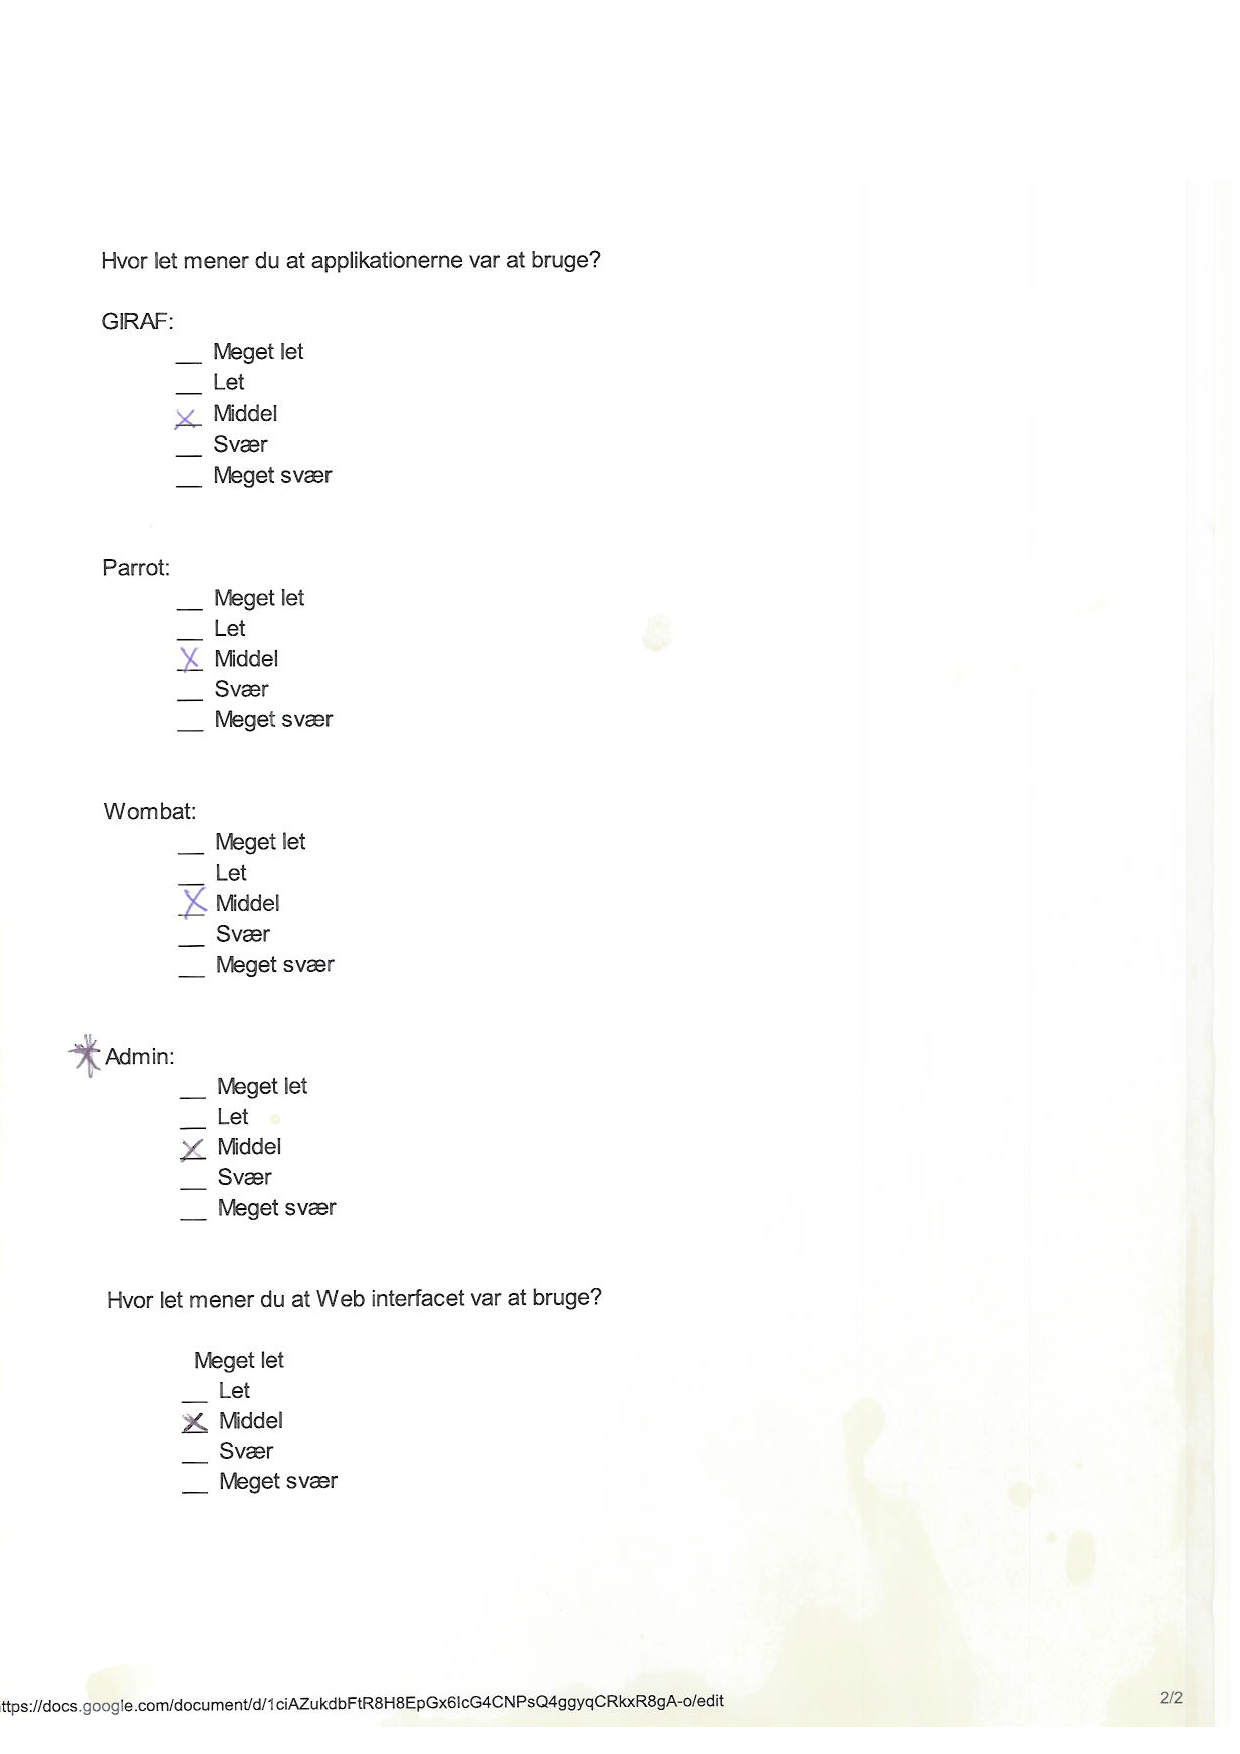
\includegraphics{Appendix/demo_d2.pdf}
	\label{fig:demo_t}
\end{figure}

\begin{figure}[h]
	\centering
		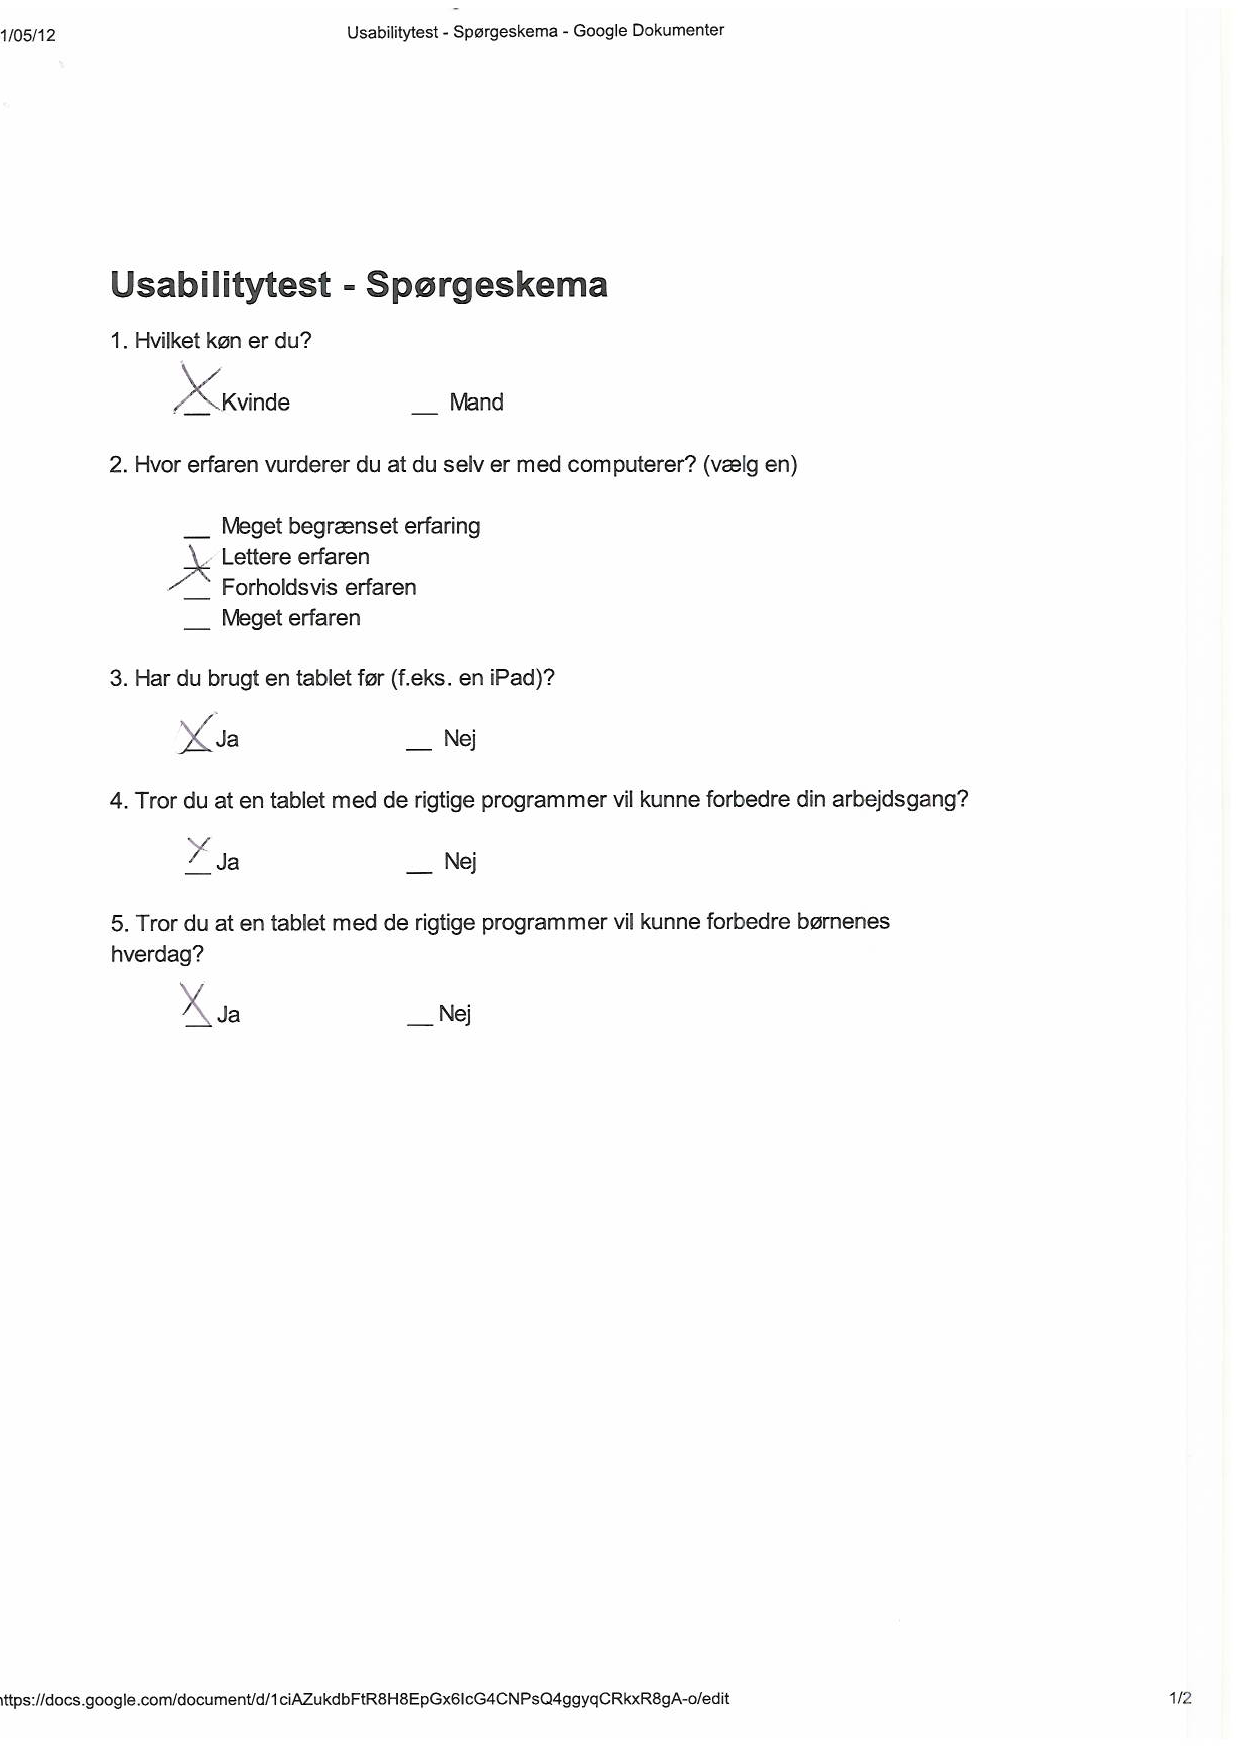
\includegraphics{Appendix/demo_m1.pdf}
	\label{fig:demo_t}
\end{figure}

\begin{figure}[h]
	\centering
		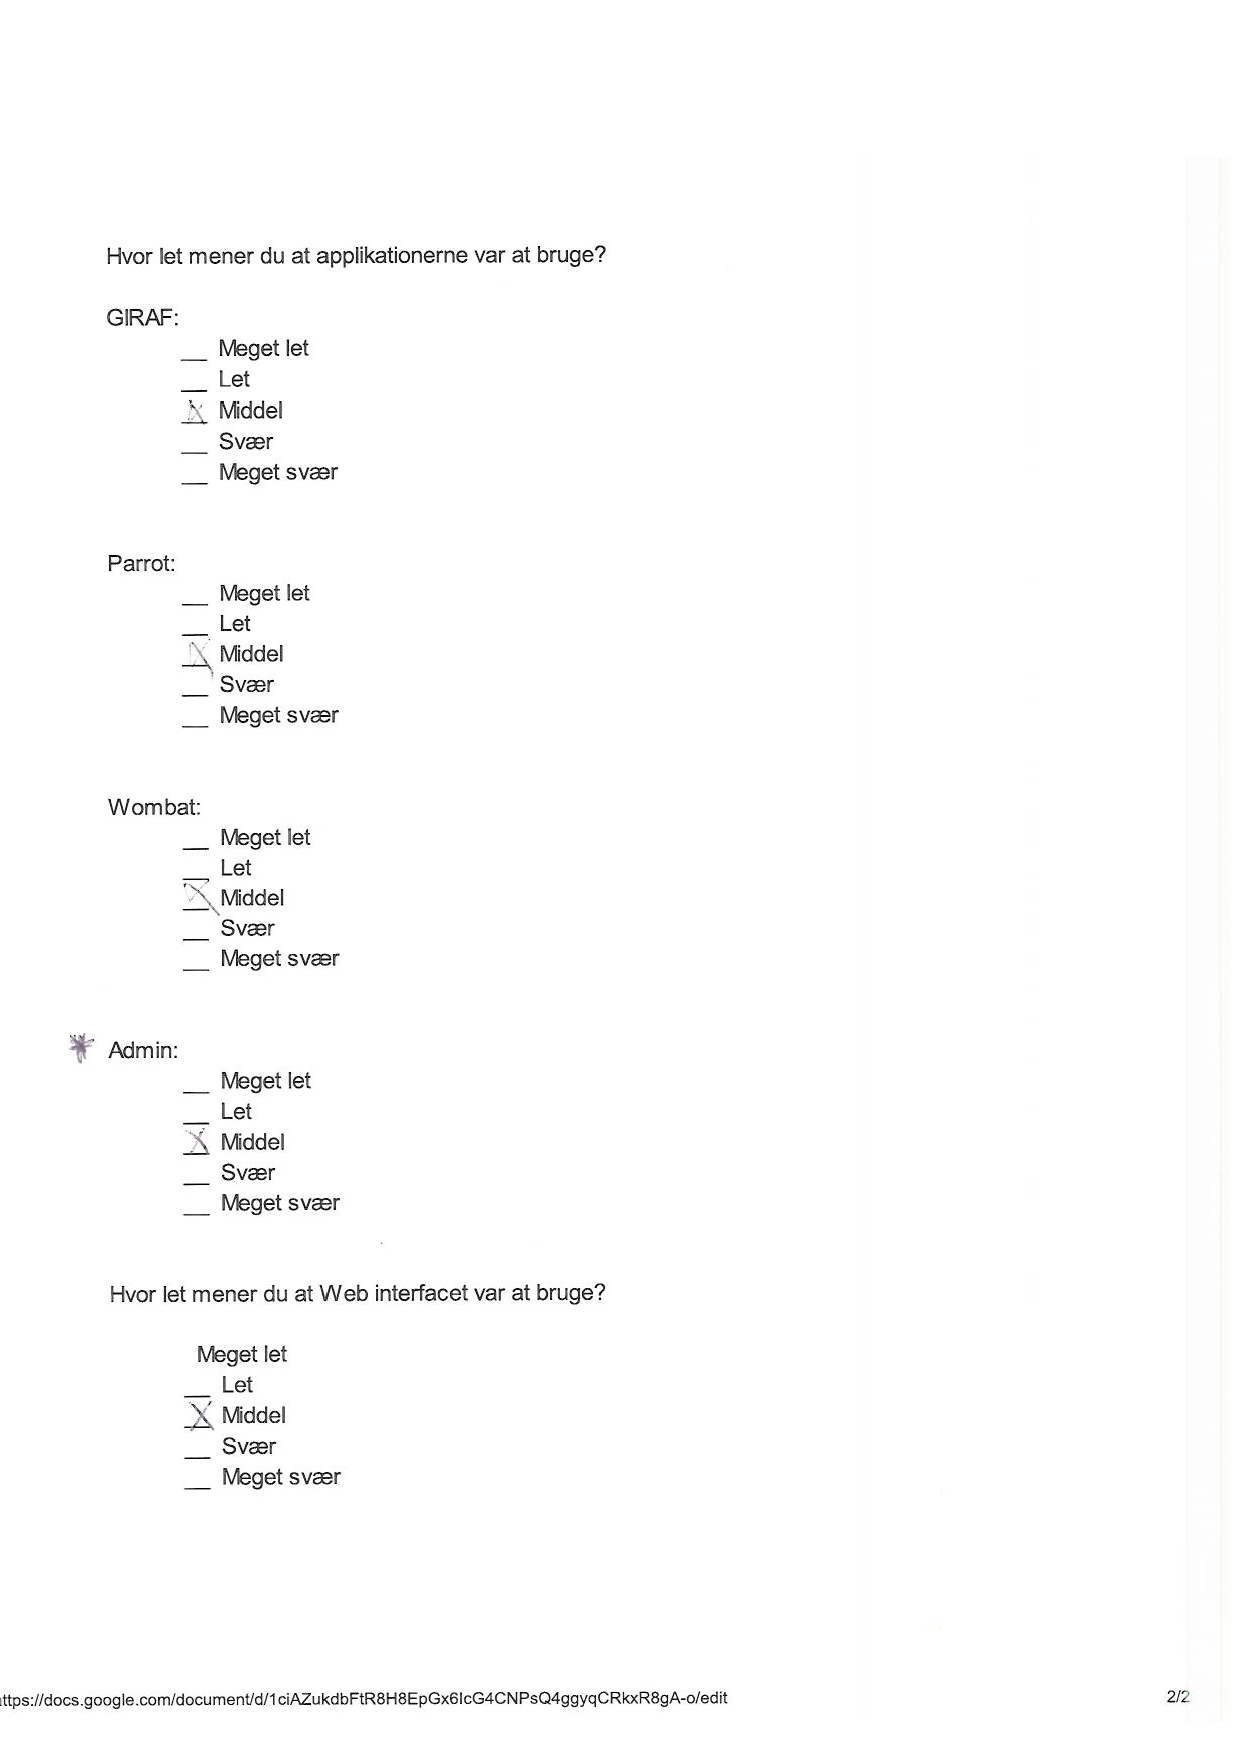
\includegraphics{Appendix/demo_m2.pdf}
	\label{fig:demo_t}
\end{figure}

\begin{figure}[h]
	\centering
		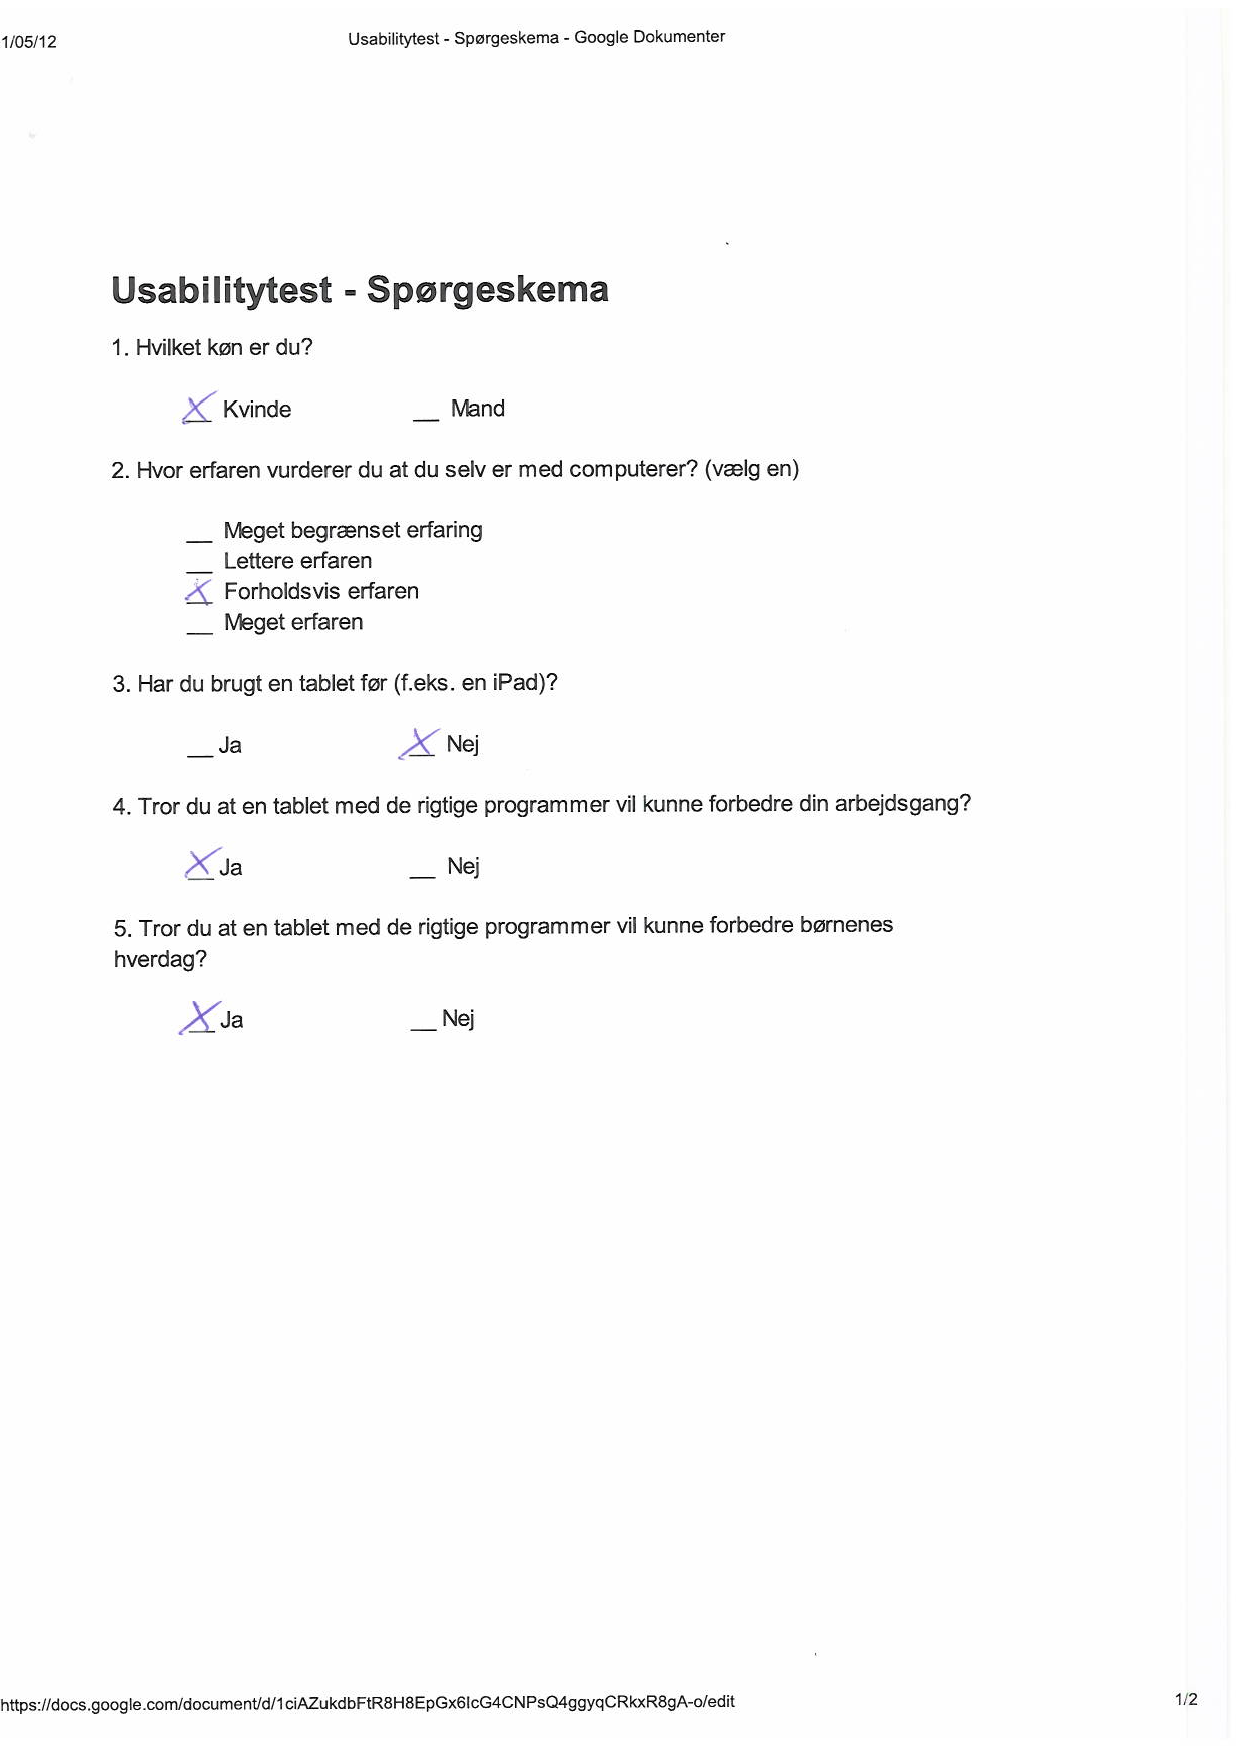
\includegraphics{Appendix/demo_t1.pdf}
	\label{fig:demo_t}
\end{figure}

\begin{figure}[h]
	\centering
		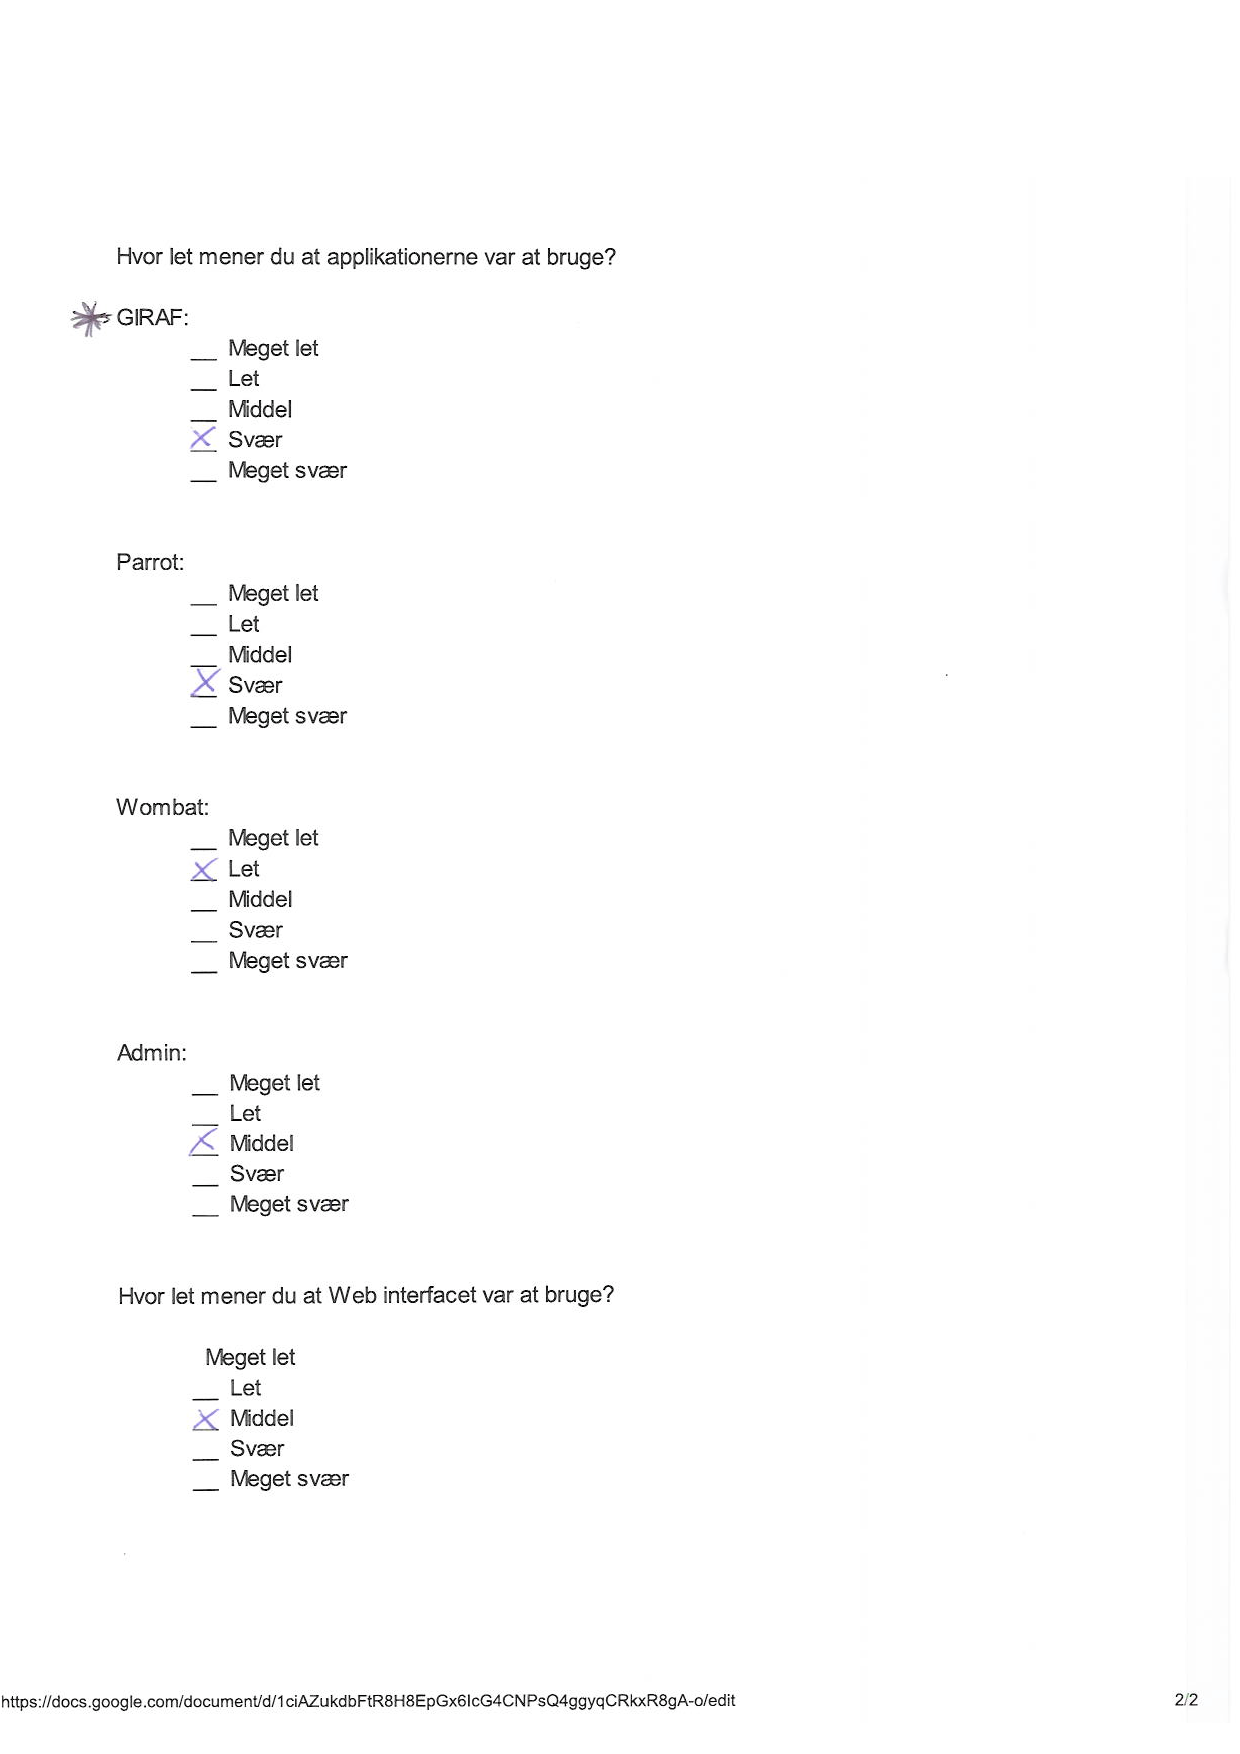
\includegraphics{Appendix/demo_t2.pdf}
	\label{fig:demo_t}
\end{figure}

\begin{figure}[h]
	\centering
		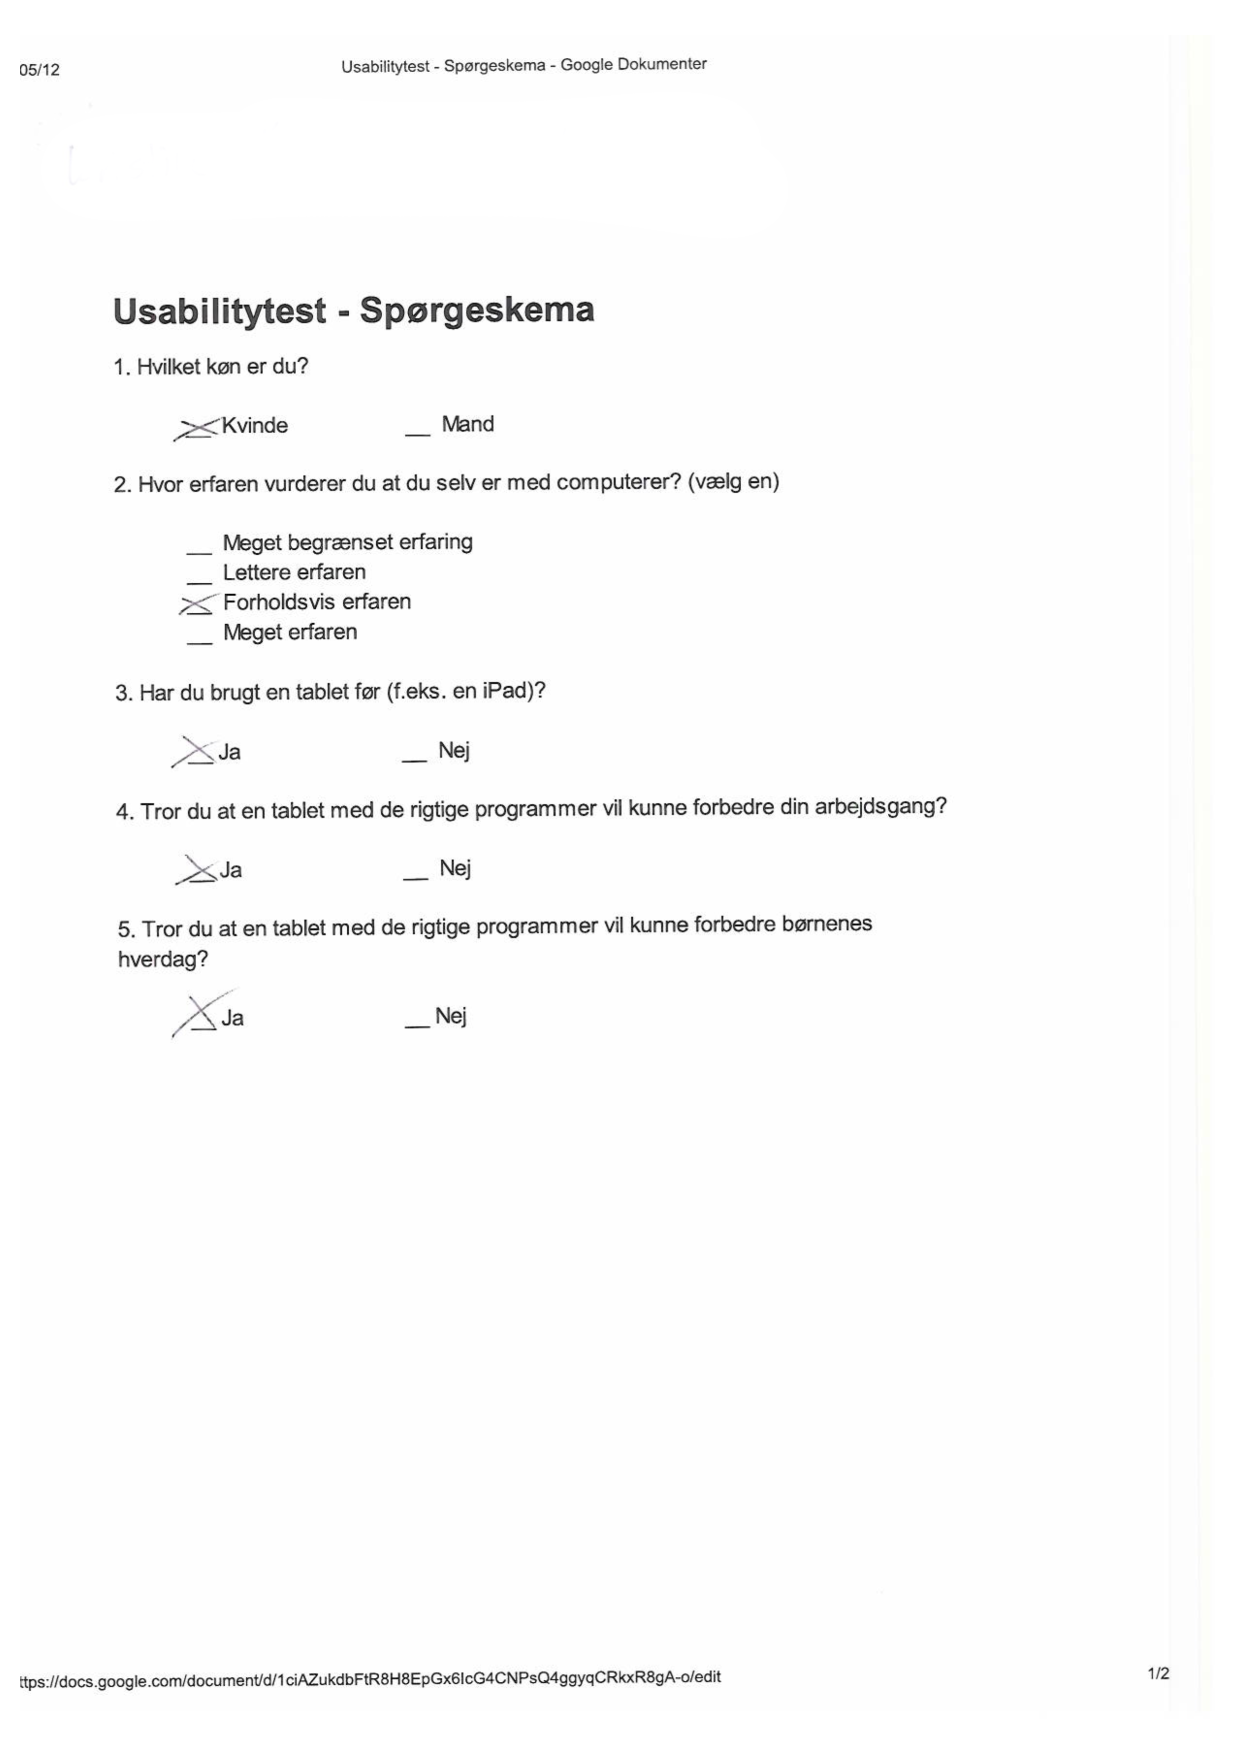
\includegraphics{Appendix/demo_k1.pdf}
	\label{fig:demo_t}
\end{figure}

\begin{figure}[h]
	\centering
		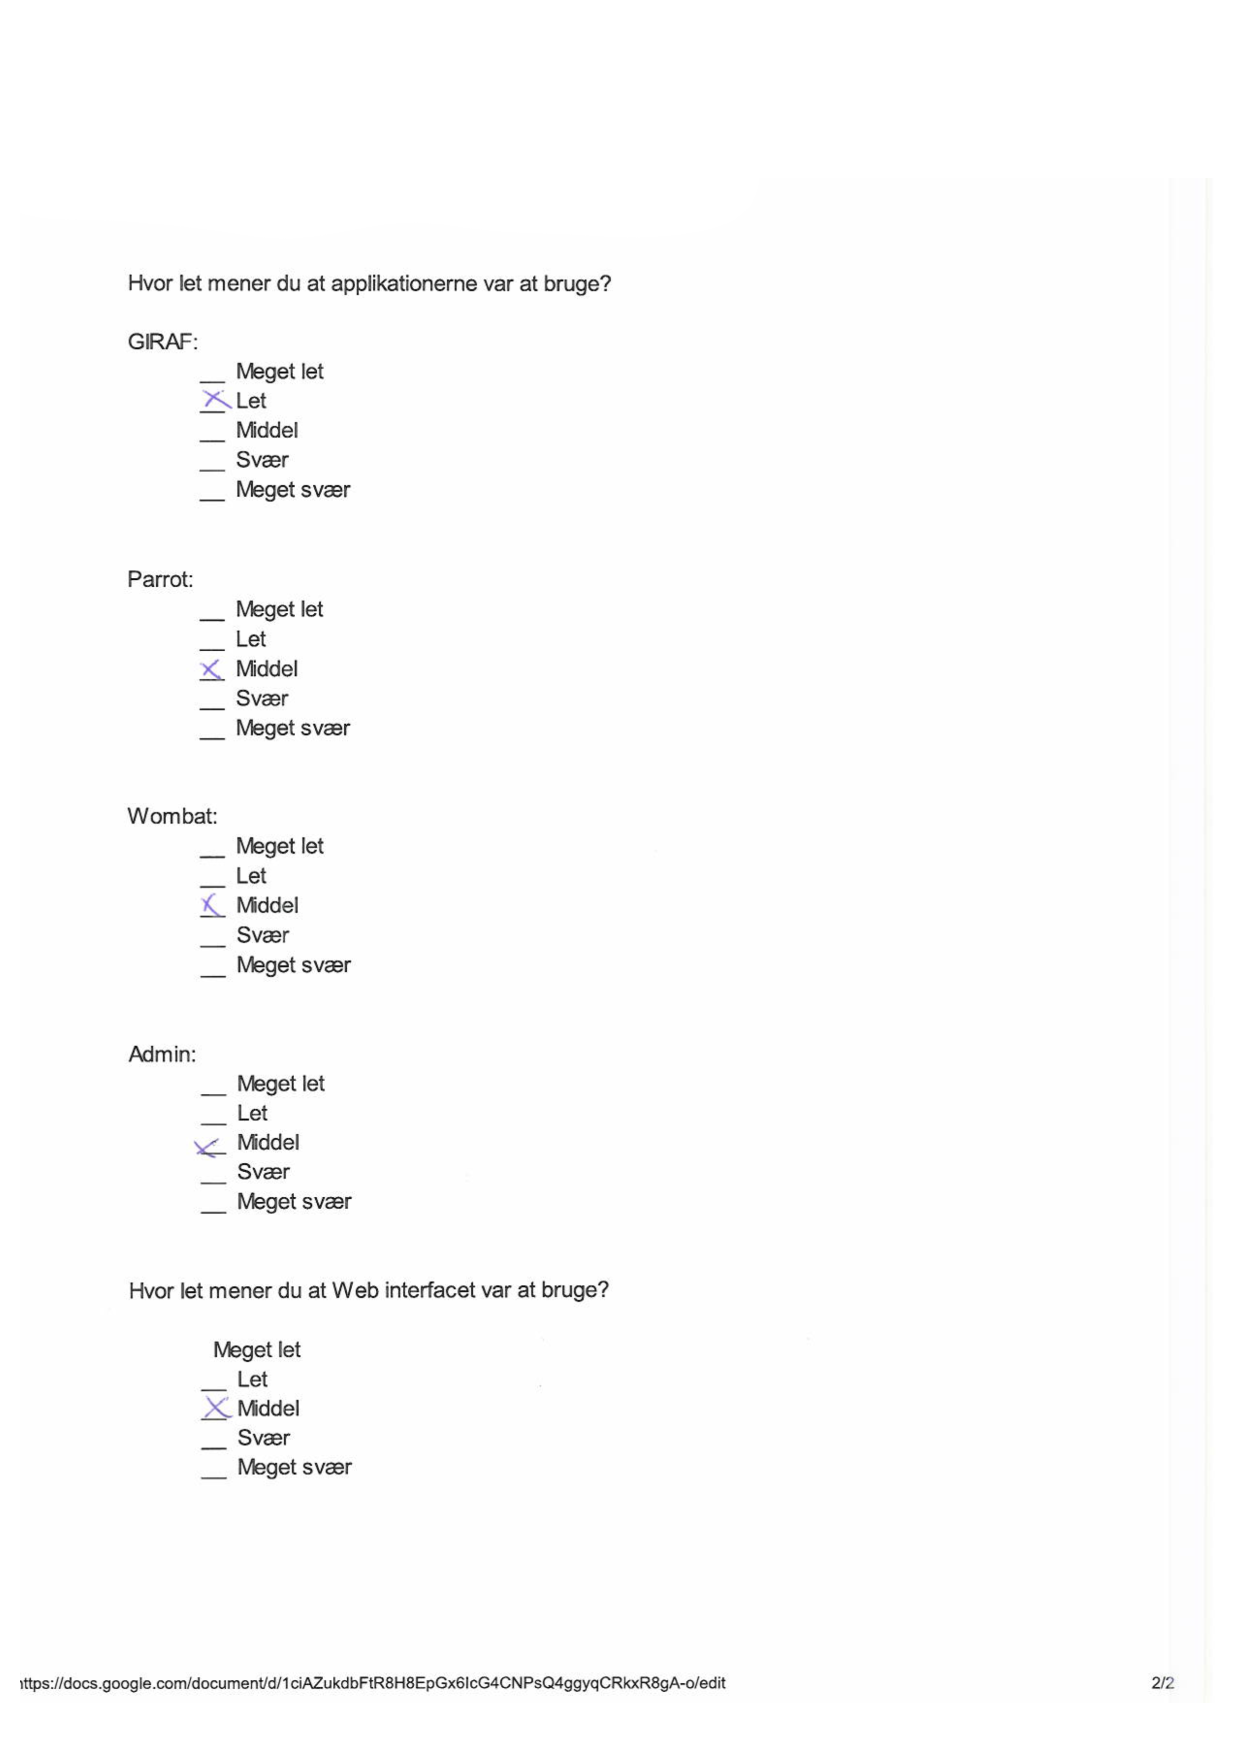
\includegraphics{Appendix/demo_k2.pdf}
	\label{fig:demo_t}
\end{figure}

\begin{figure}[h]
	\centering
		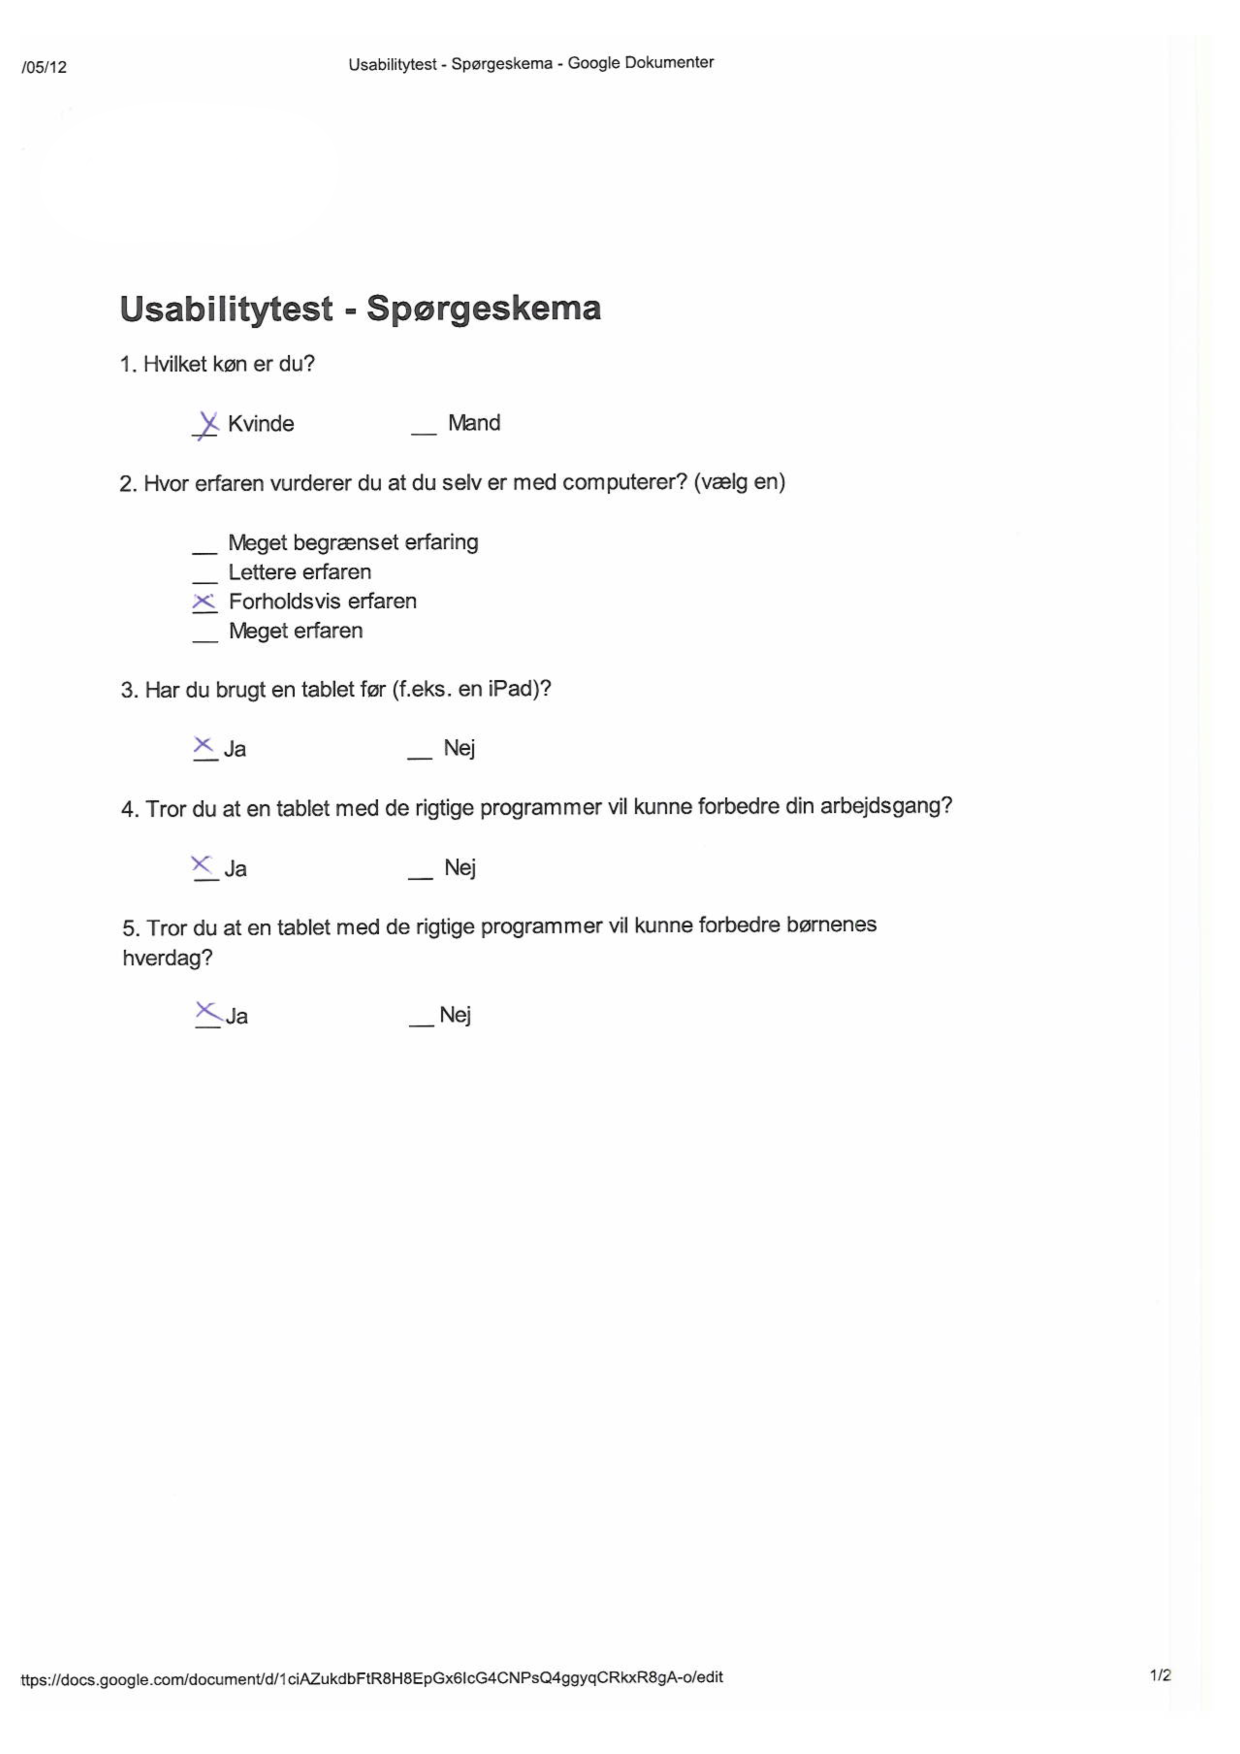
\includegraphics{Appendix/demo_ma1.pdf}
	\label{fig:demo_t}
\end{figure}

\begin{figure}[h]
	\centering
		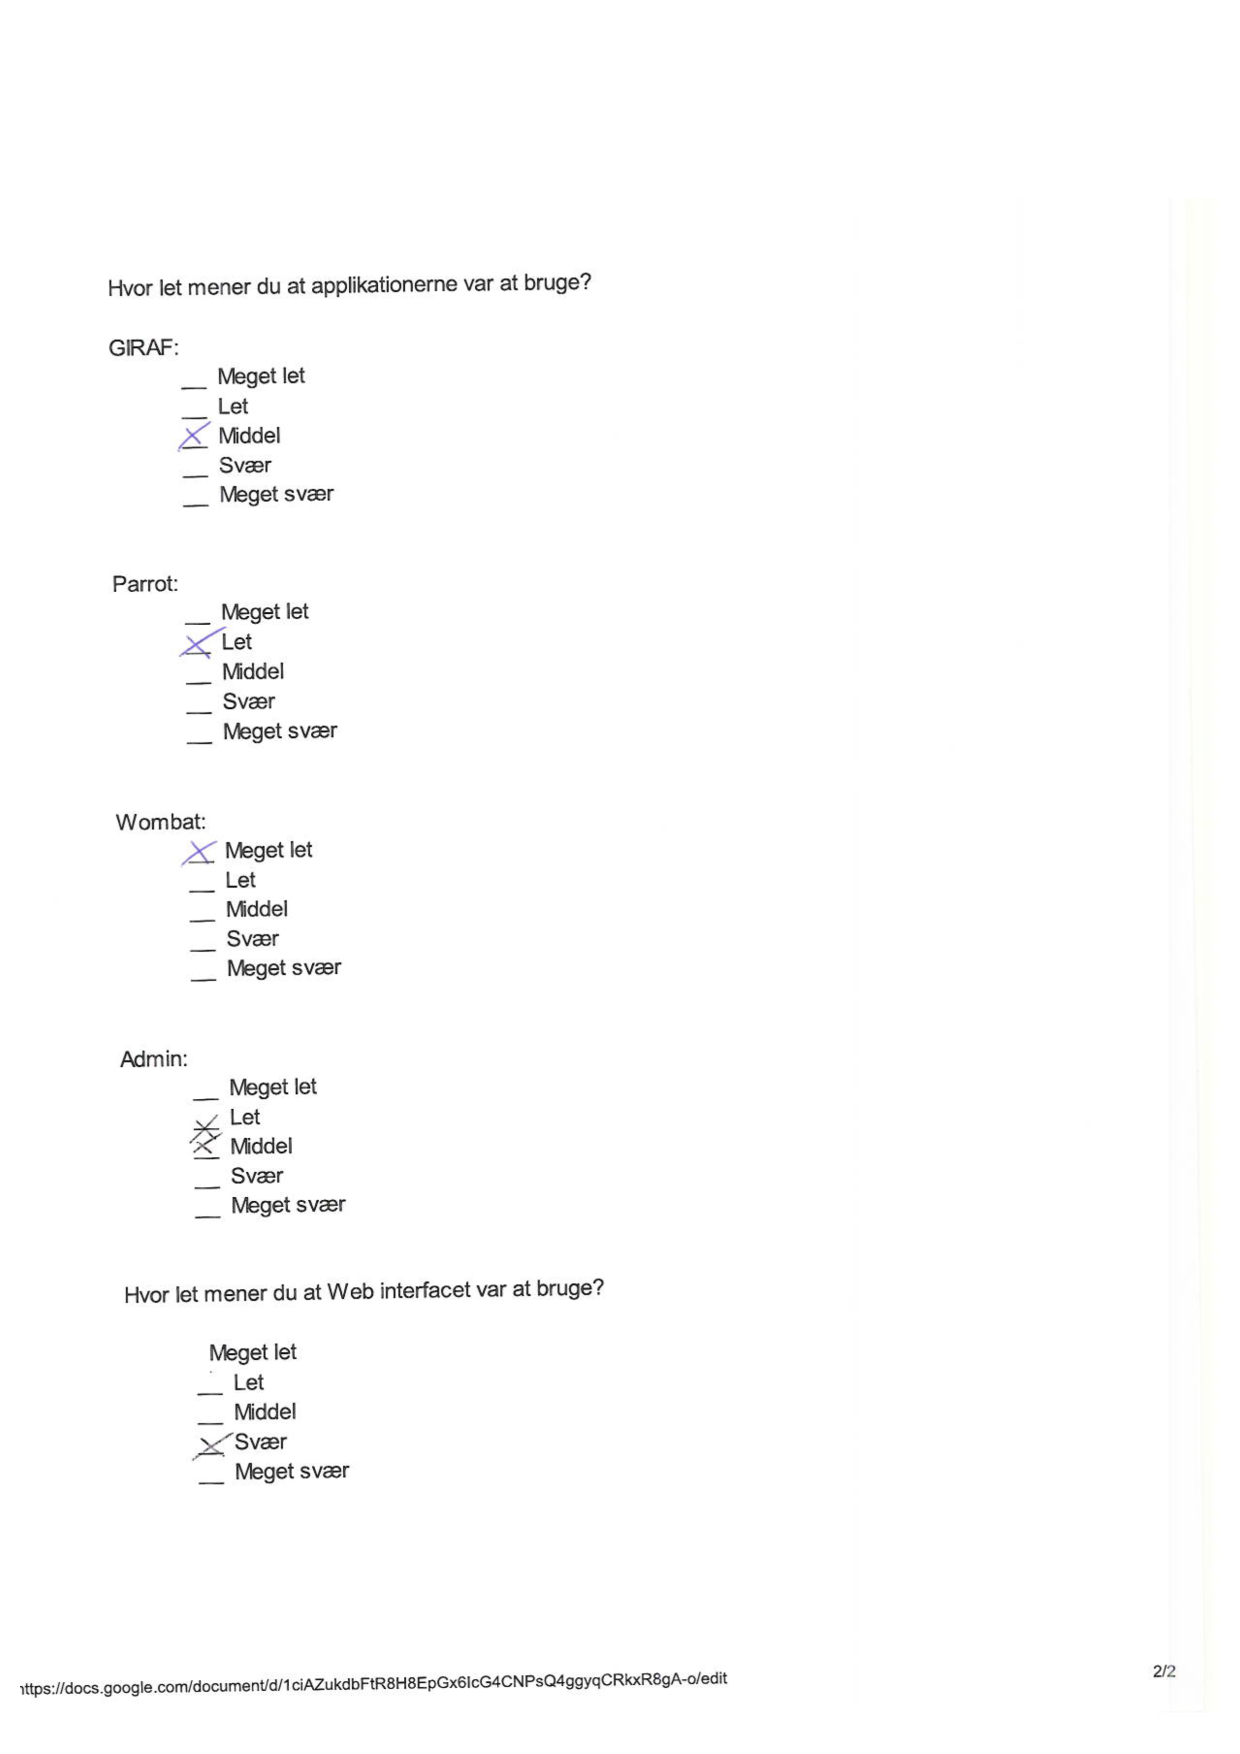
\includegraphics{Appendix/demo_ma2.pdf}
	\label{fig:demo_t}
\end{figure}

% ------ Notes from interview with Mette Als Andreasen from Birken --------- %
	\section{Notes from Interview}
\label{InterviewMette}
\textit{This is notes from an interview with Mette Als Andreasen, an educator at Birken in Langholt, Denmark.}

N�r tiden l�ber ud (kristian har tage et billede):\\
F�rdig - symbol\\
G� til skema - symbol\\
Taget fra boardmaker\\

Kunne v�re godt hvis man kunne s�tte egne billeder ind som start/stop symboler.\\


R�d farve $=$ nej, stop, aflyst.\\

De har s�dan et ur p� 60 minutter hvor tid tilbage er markeret med r�d, og s� bipper den lige kort n�r den er f�rdig.\\
  Det ville v�re fint hvis de kunne bruge sort/hvid til dem der ikke kan h�ndtere farver, men ogs� kan v�lge farver.\\

Stop-ur:\\
en fast timer p� 60 minutter $+$ en customizable som ikke ser helt magen til ud, som f.eks, kan v�re p� 5, 10 eller 15 minutter for en hel cirkel.\\

timeglas:\\
skift farve p� timeglassene, men ikke n�dvendigvis g�re dem st�rre. Kombinere med mere/mindre sand. Eventuelt kombinere med et lille digitalt ur, til dem der har brug for det, skal kunne sl�es til og fra.\\

Dags-plan:\\
ikke s�rlig relevant til de helt sm� og ikke s�rligt velfungerende b�rn. Men kunne v�re rigtig godt til de lidt �ldre.\\
   En plan g�r oppefra og ned, og hvis der s� skal specificeres noget ud til aktiviteterne, s� er det fra venstre mod h�jre ud fra det nedadg�ende skema.\\

Til parrot:\\
Godt med rigtige billeder af tingene, som p�dagogerne selv kan tage, eventuelt ogs� af aktiviteter, s� pedagogerne kan have billeder af aktiviter som de kan liste efter skeamet.\\

Der var mange skemaer rundt omkring, og der henviser det sidste billede i r�kken til n�ste skema, som h�nger f.eks. p� badev�relset eller i garderoben.



%%%%%%%%%%%%%%%%%%%%%%%%%%%%%%%%%%%%%%
% ------ Individual report --------- %

% ------ paper prototypes --------- %
\section{Paper Prototypes}
	\label{sec:paper_prot}

	\begin{figure}[H]
		\centering
			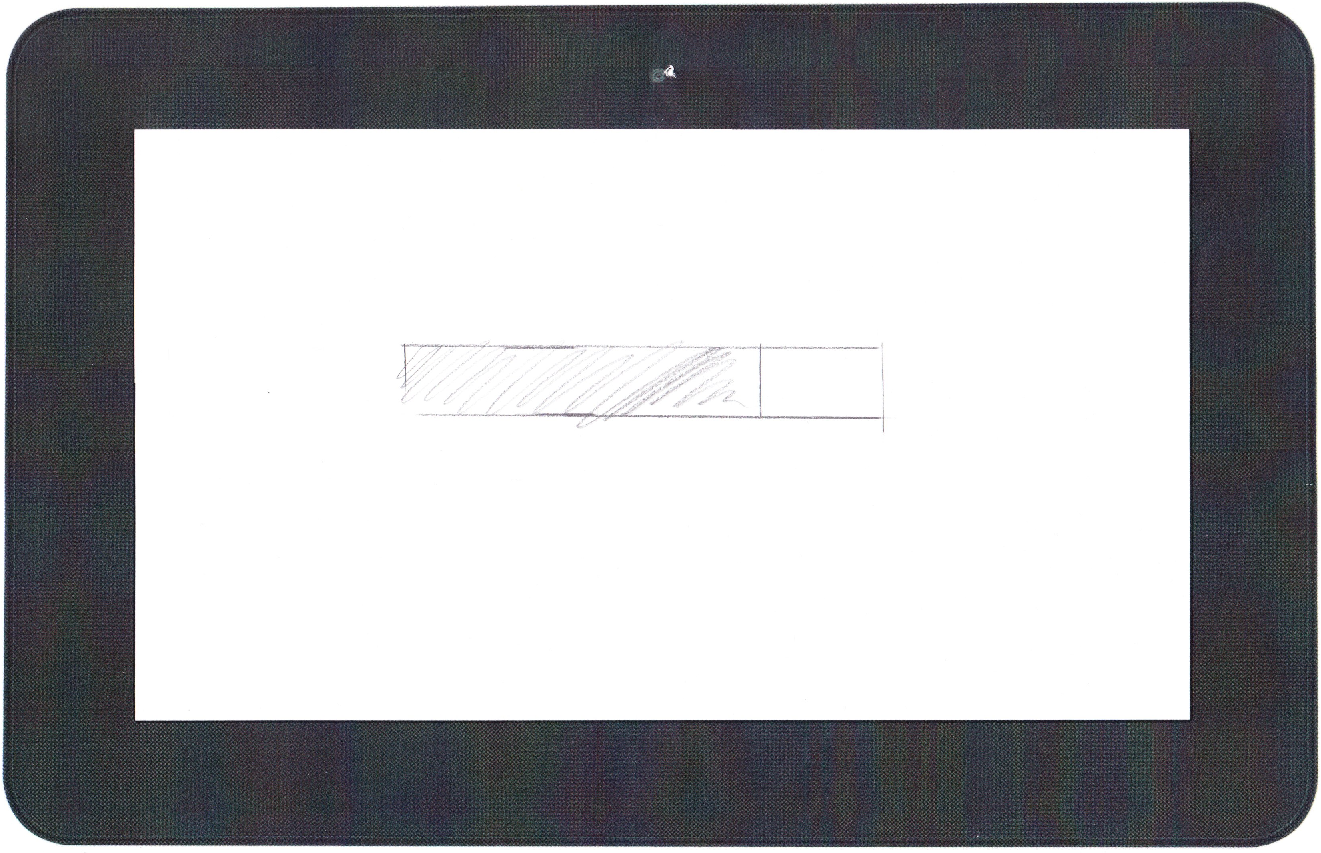
\includegraphics[width=\textwidth]{Images/paper_prototype/timer_1.png}
				\caption{Scan of a paper prototype of a single progress bar timer.}
		\label{fig:pap_prot_progbar}
	\end{figure}
	
	\begin{figure}[H]
		\centering
			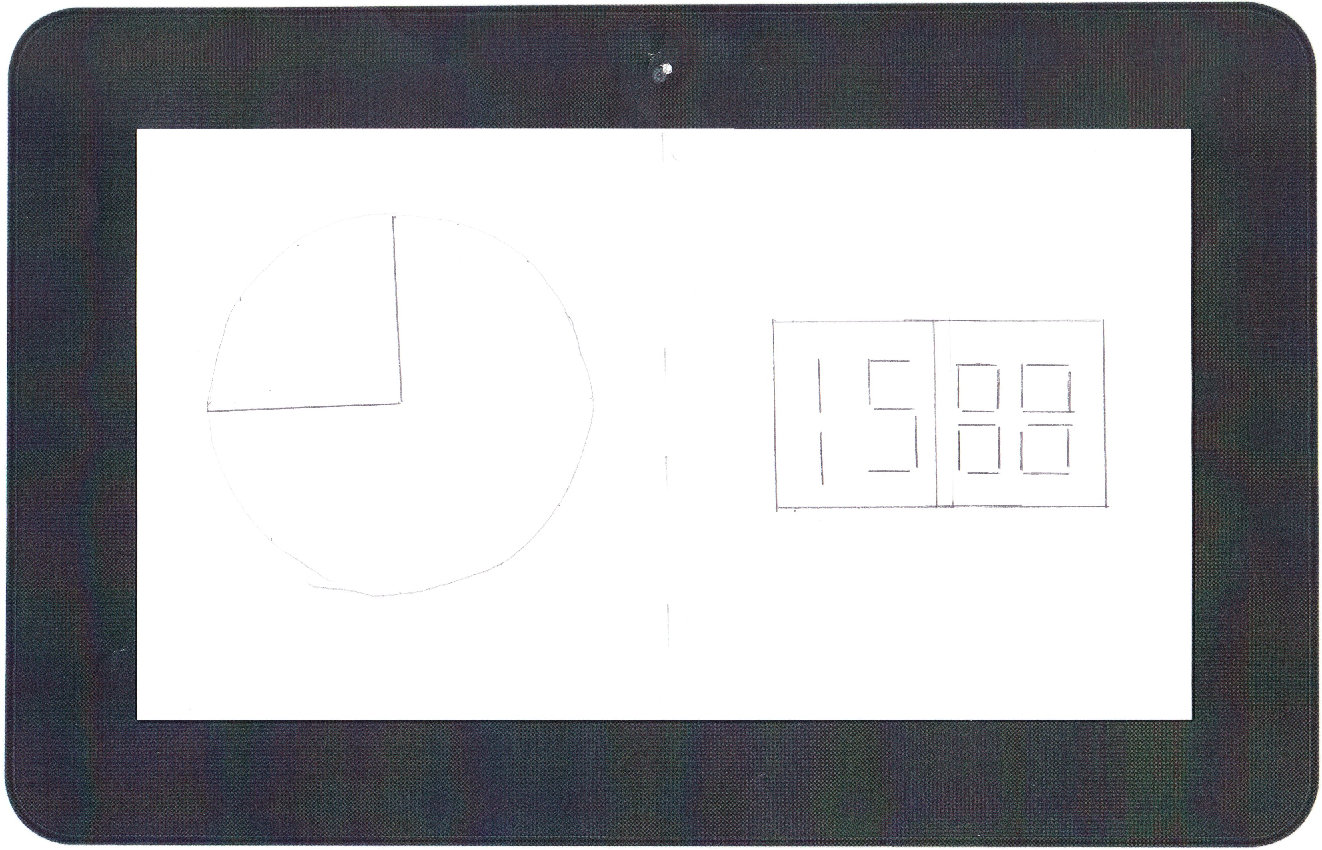
\includegraphics[width=\textwidth]{Images/paper_prototype/timer_2.png}
				\caption{Scan of a paper prototype of a double timer.}
		\label{fig:pap_prot_timedoub1}
	\end{figure}

	\begin{figure}[H]
		\centering
			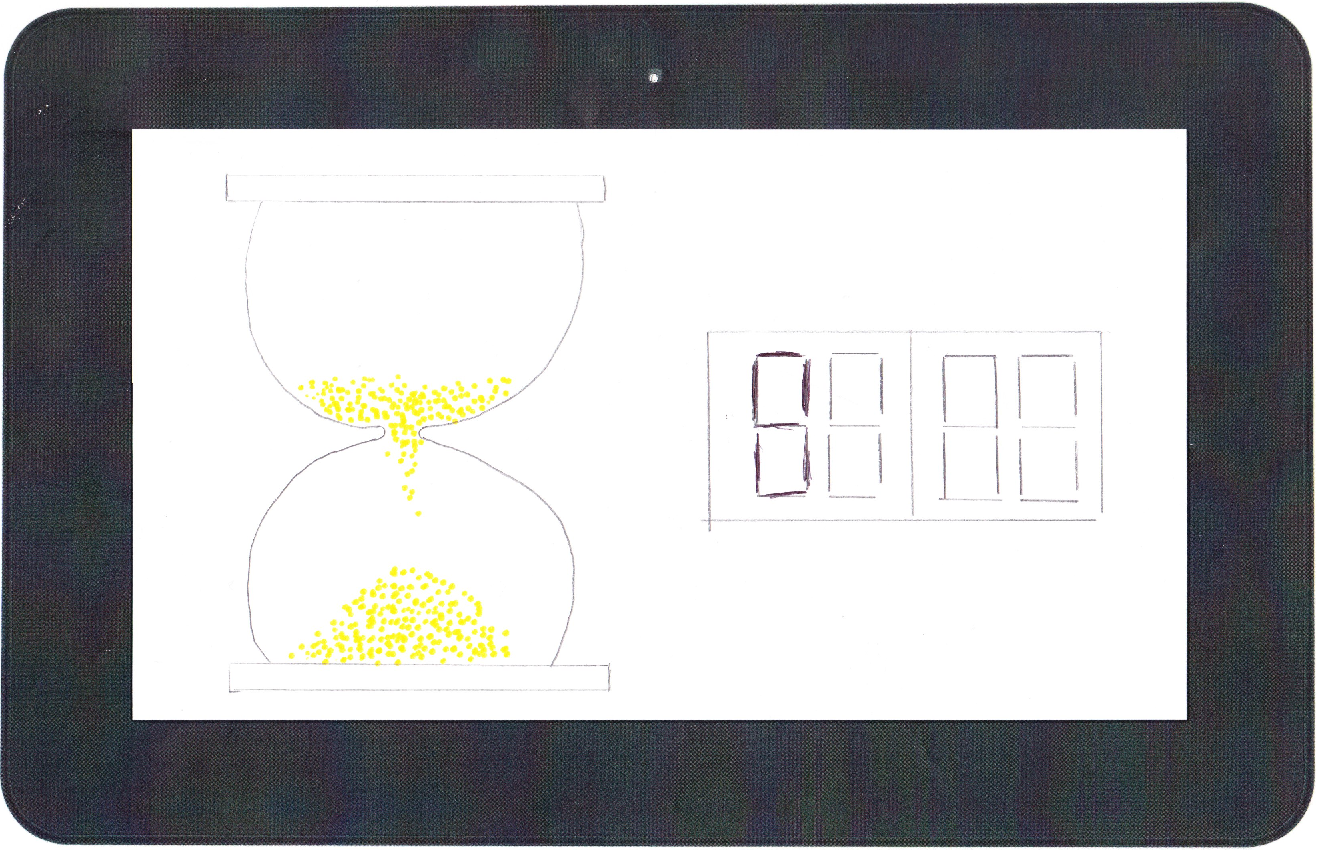
\includegraphics[width=\textwidth]{Images/paper_prototype/timer_3.png}
				\caption{Scan of a paper prototype of another double timer.}
		\label{fig:pap_prot_timedoub2}
	\end{figure}

	\begin{figure}[H]
		\centering
			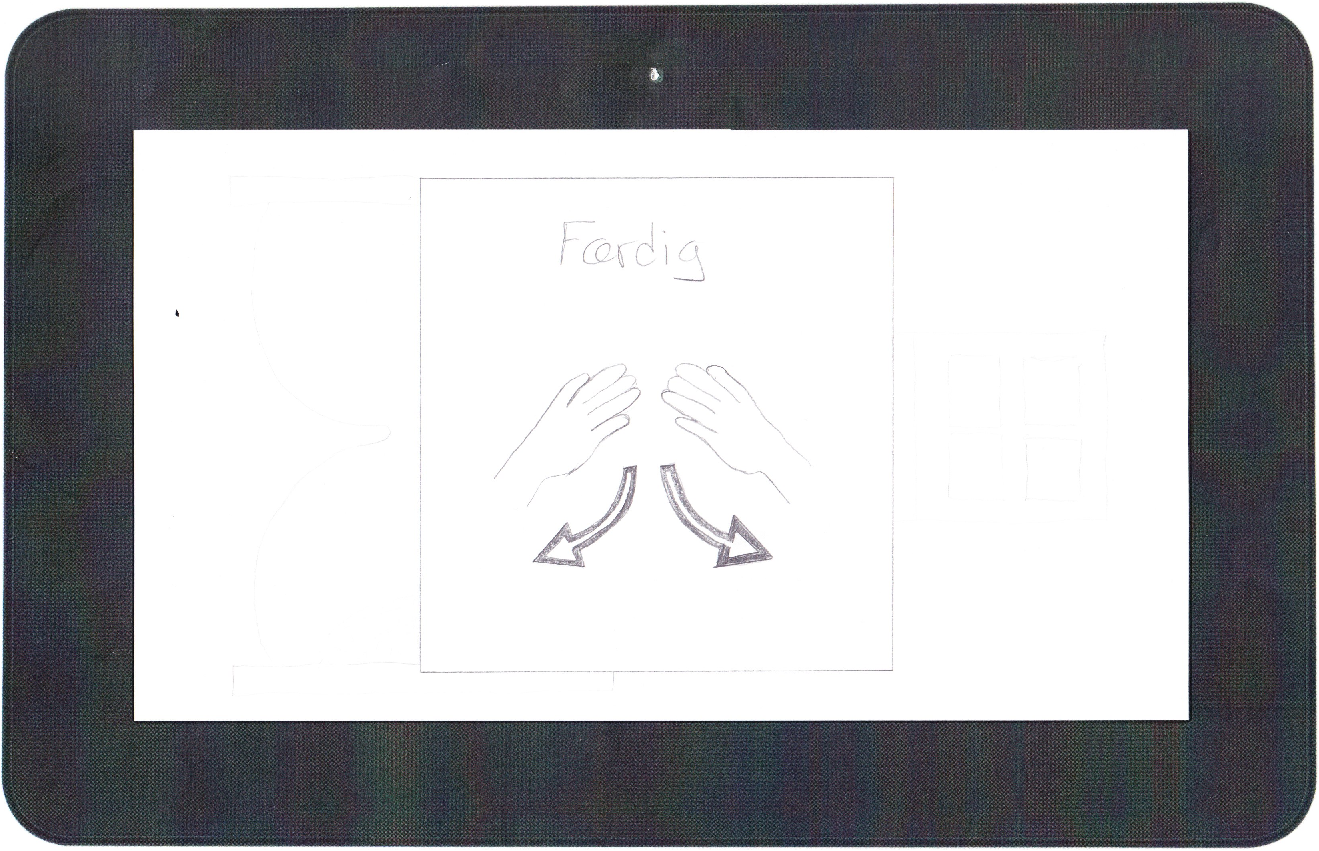
\includegraphics[width=\textwidth]{Images/paper_prototype/done.png}
				\caption{Scan of a paper prototype of the "Done" screen shown when the time has run out.}
		\label{fig:pap_prot_donescr}
	\end{figure}

% ------ burndown charts --------- %
\section{Sprint Burndown Charts and Backlogs}
\label{sec:burn_back}
	
	\begin{figure}[H]
		\centering
			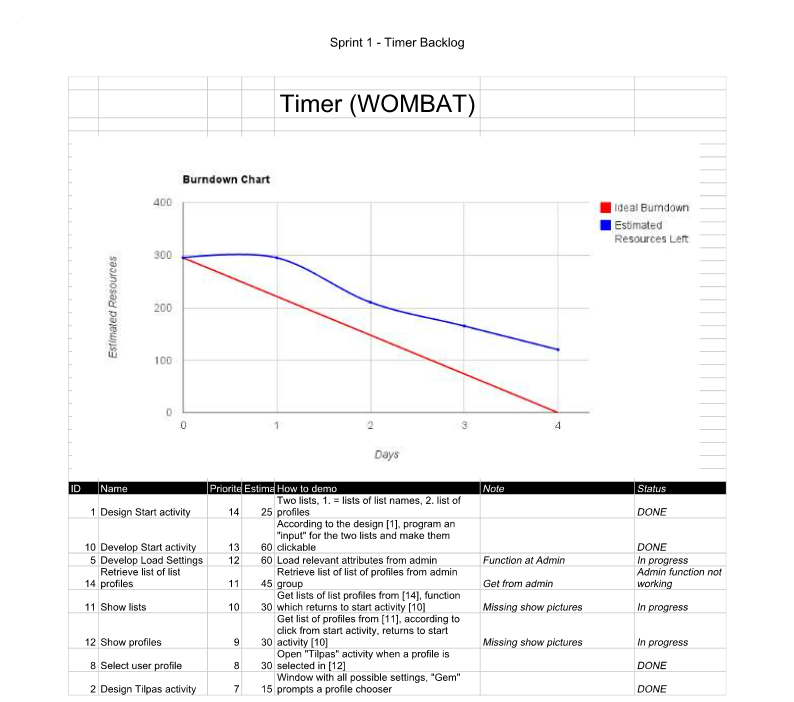
\includegraphics[width=\textwidth]{Development/burndown_charts/Sprint_1.png}
				\caption{Sprint 1.}
		\label{fig:sprint1}
	\end{figure}
	
	\begin{figure}[H]
		\centering
			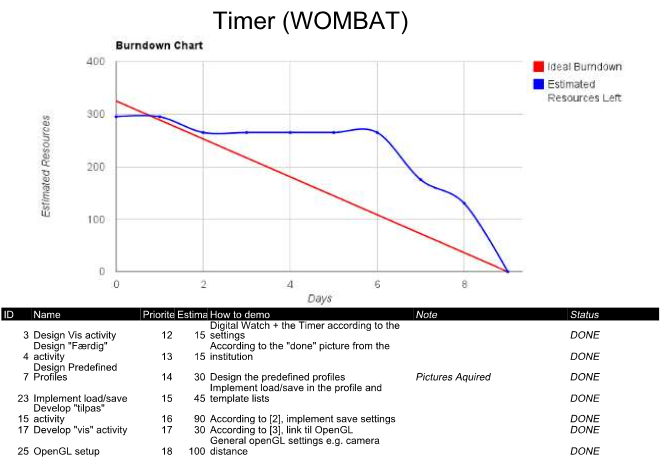
\includegraphics[width=\textwidth]{Development/burndown_charts/Sprint_2.png}
				\caption{Sprint 2.}
		\label{fig:sprint2}
	\end{figure}
	
	\begin{figure}[H]
		\centering
			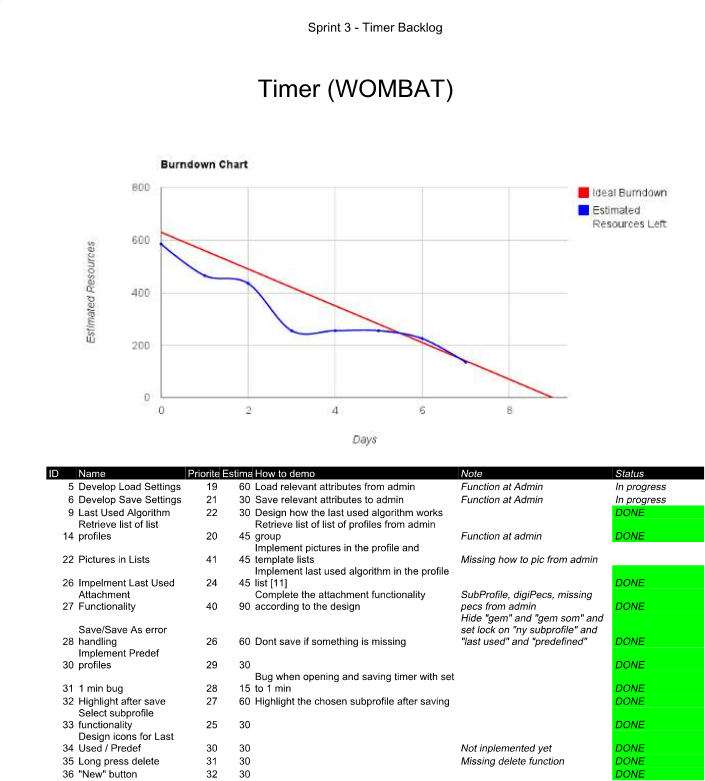
\includegraphics[width=\textwidth]{Development/burndown_charts/Sprint_3.png}
				\caption{Sprint 3.}
		\label{fig:sprint3}
	\end{figure}
	
	\begin{figure}[H]
		\centering
			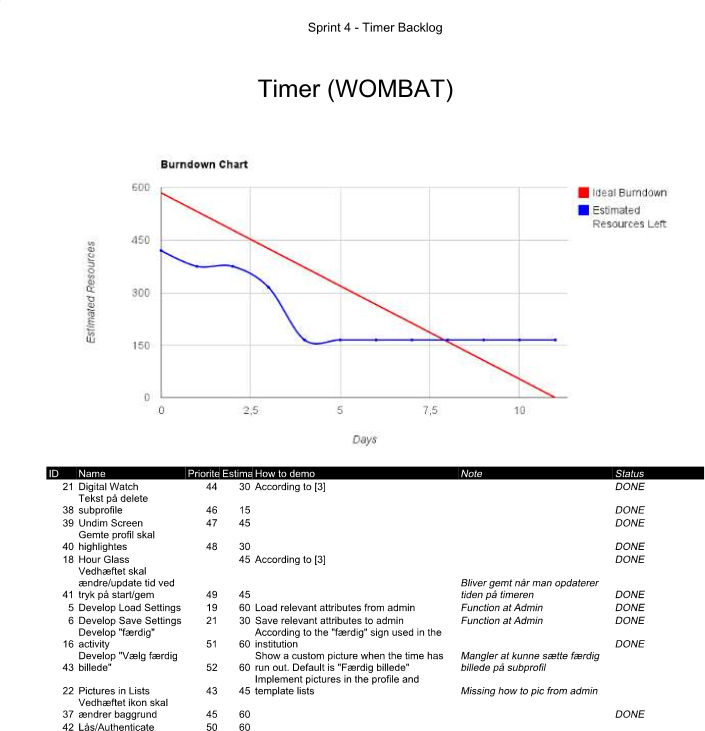
\includegraphics[width=\textwidth]{Development/burndown_charts/Sprint_4.png}
				\caption{Sprint 4.}
		\label{fig:sprint4}
	\end{figure}
	
	\begin{figure}[H]
		\centering
			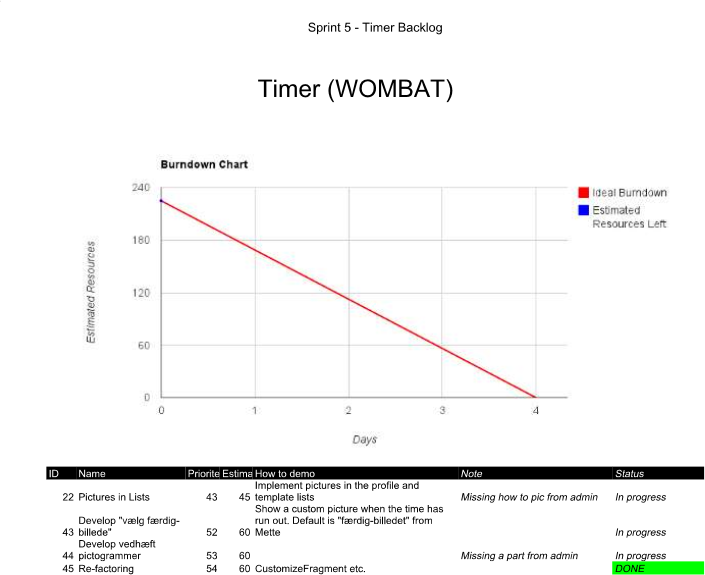
\includegraphics[width=\textwidth]{Development/burndown_charts/Sprint_5.png}
				\caption{Sprint 5.}
		\label{fig:sprint5}
	\end{figure}
	
	\begin{figure}[H]
		\centering
			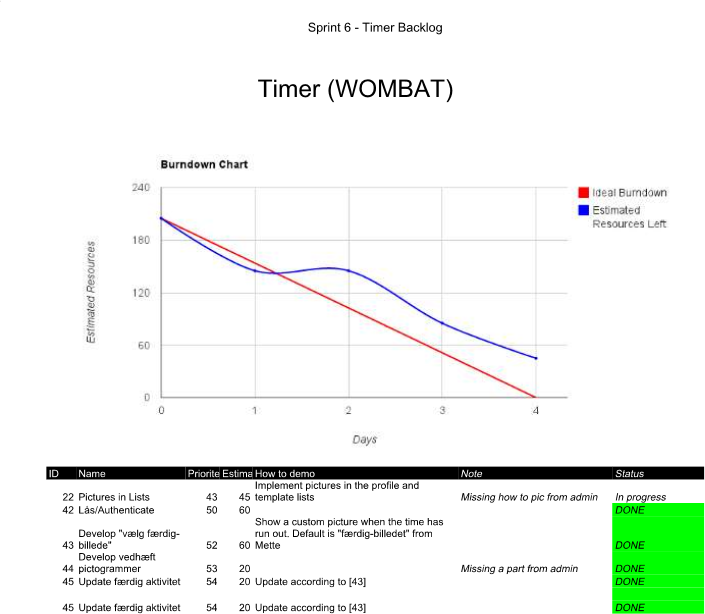
\includegraphics[width=\textwidth]{Development/burndown_charts/Sprint_6.png}
				\caption{Sprint 6.}
		\label{fig:sprint6}
	\end{figure}
	
	
	\begin{figure}[H]
		\centering
			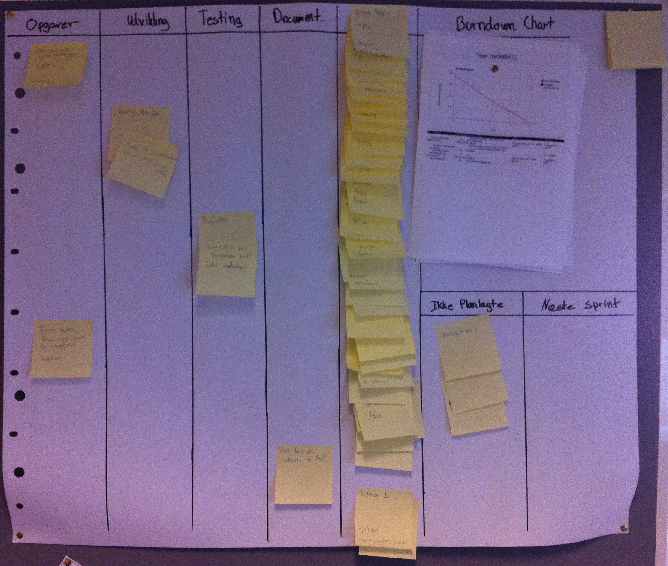
\includegraphics[width=\textwidth]{Images/burndown.png}
				\caption{Picture of our burndownchart and list of assignments. Used to manage the total project backlog.}
		\label{fig:burn}
	\end{figure}
	
% ------ SWOT - development tools --------- %
\section{Analysis of the Project}
\label{sec:swot}
\begin{center}
		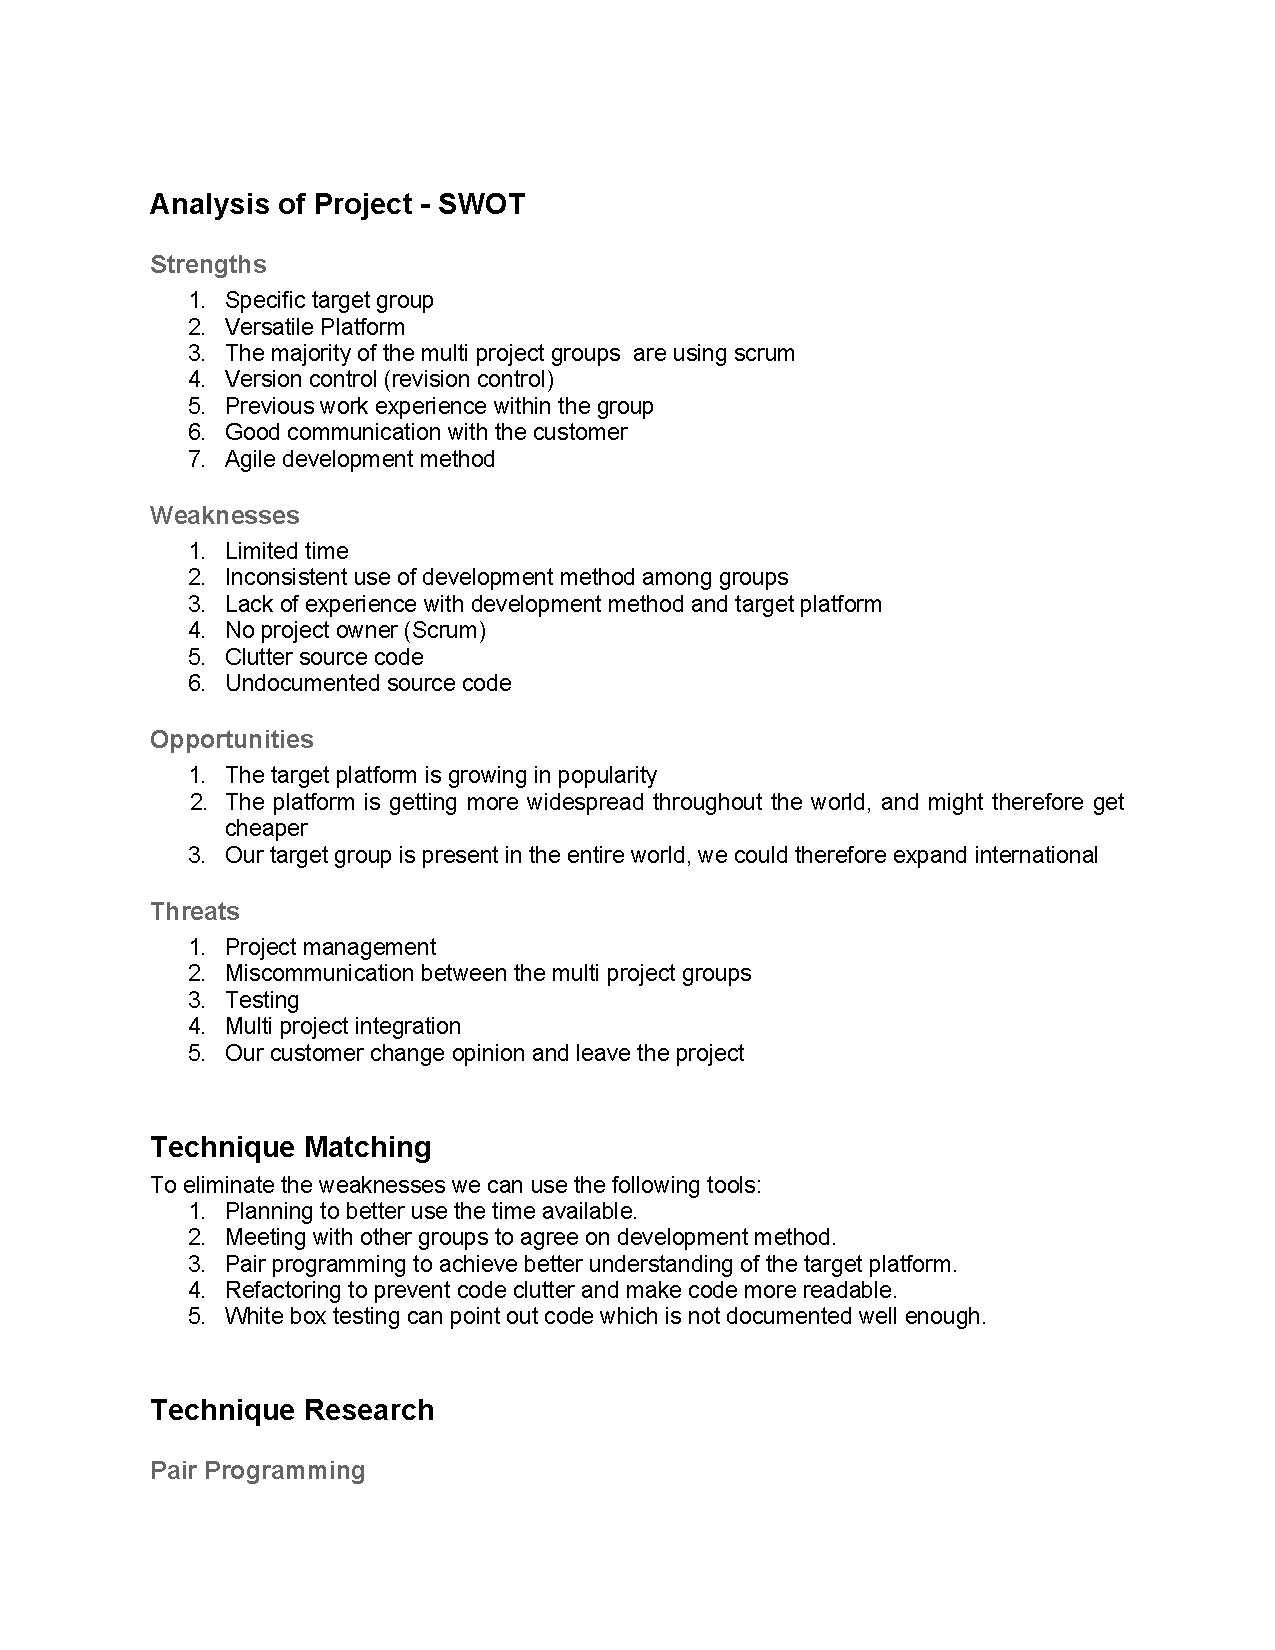
\includegraphics[width=\textwidth]{Appendix/SWOT.pdf}
		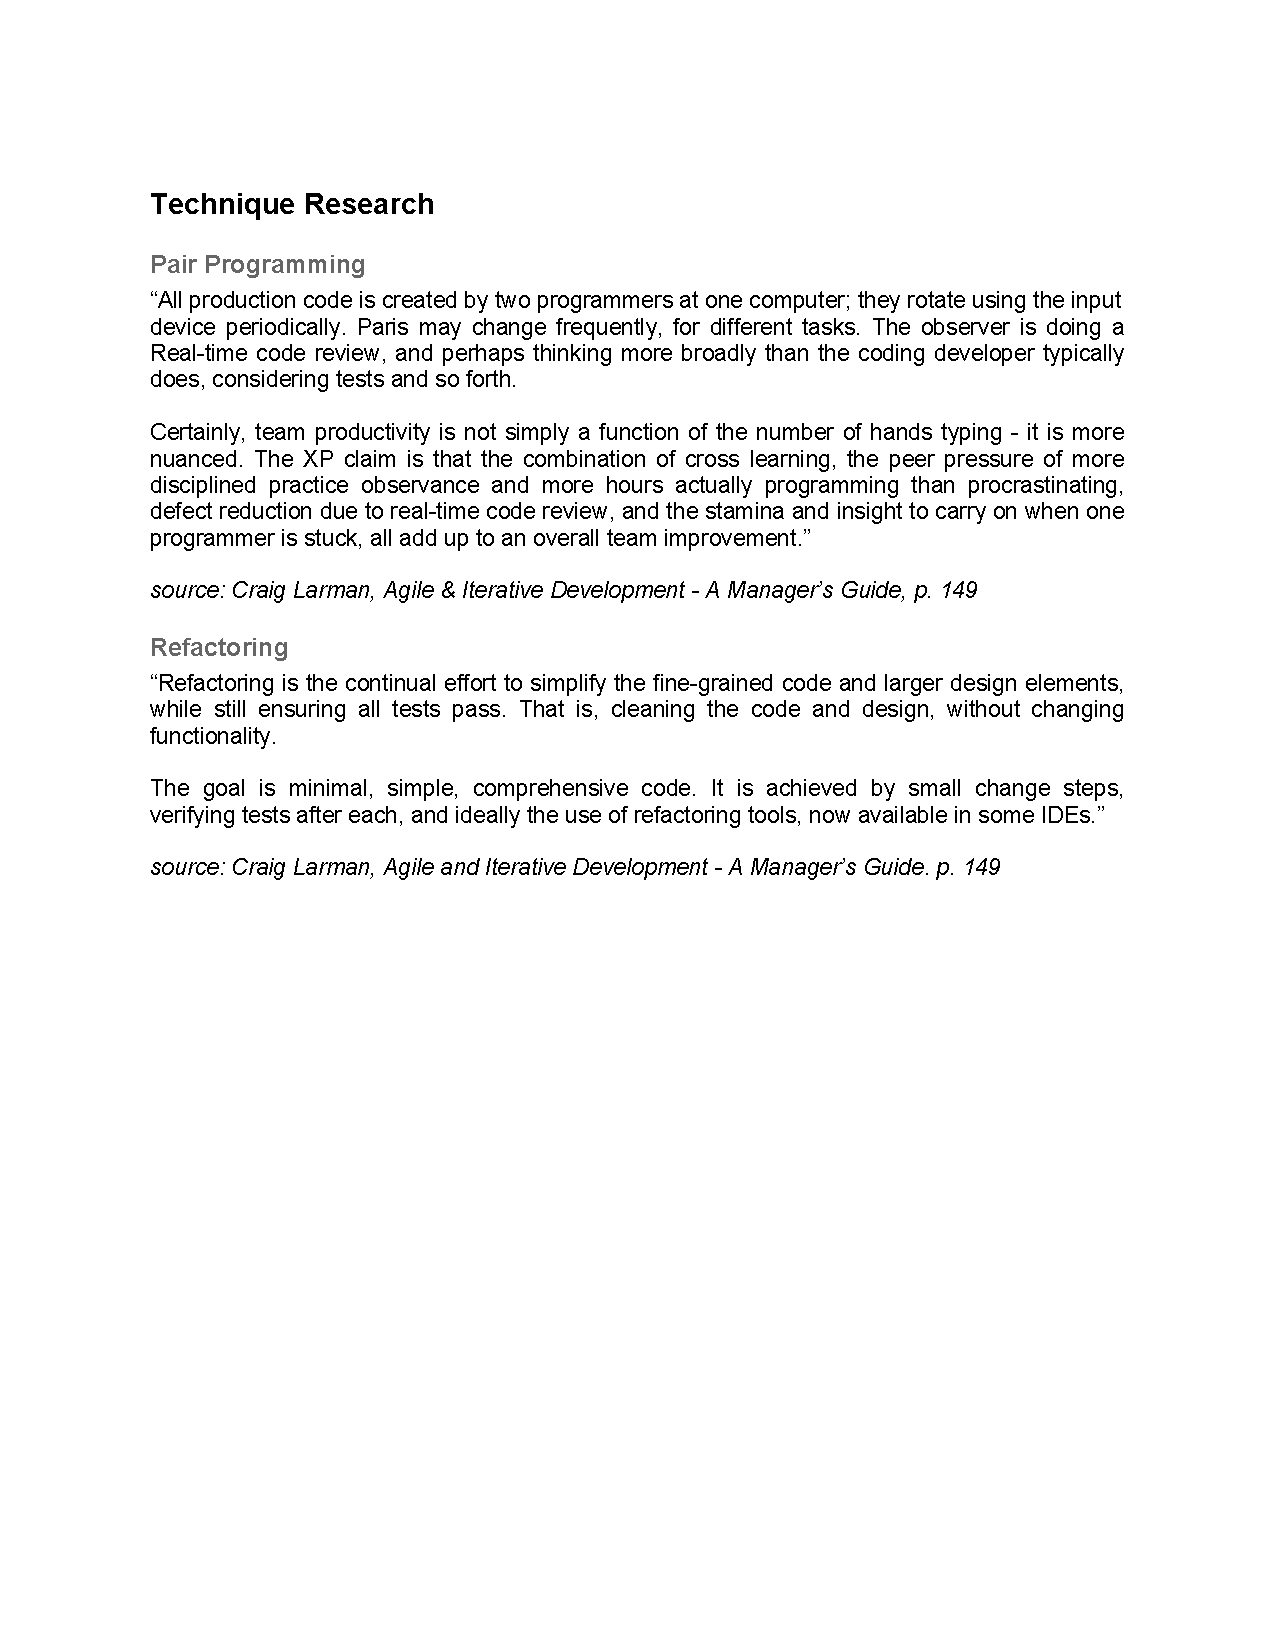
\includegraphics[width=\textwidth]{Appendix/SWOT_2.pdf}
	\end{center}

% ------ acceptance test diary --------- %
	\section{Acceptance Test Diary}
	\label{sec:acceptance}
	\begin{center}
		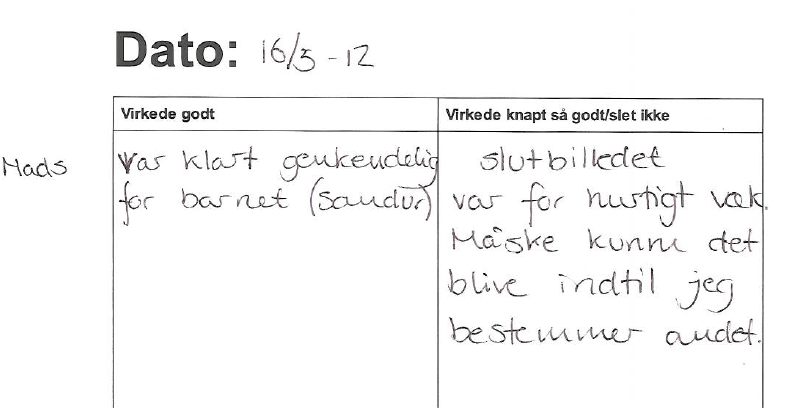
\includegraphics[width=\textwidth]{Development/Acceptance_diary/Diary_1.png}
		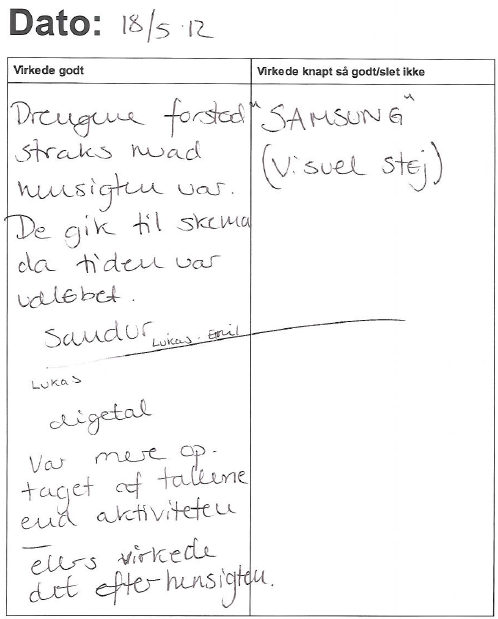
\includegraphics[width=\textwidth]{Development/Acceptance_diary/Diary_2.png}
	\end{center}
	
	\begin{figure}[H]
		\centering
			
\includegraphics[width=\textwidth]{Images/Screenshots/last_used.png}
				\caption{Scan of a paper prototype of the "Done" screen shown when the time has run out.}
		\label{fig:last_used_screenshot}
	\end{figure}
	
% ------ How to WOMBAT... --------- %
\section{WOMBAT Setup for Eclipse}
To fetch the released code from SVN, make a checkout to \url{https://sw6-2012.googlecode.com/svn/tags/wombat/}, previous versions of the project, reports, and the wiki can be found by making a checkout to \url{https://sw6-2012.googlecode.com/svn/}.
The folders on SVN contains the following:

	\begin{itemize}
		\item \textit{trunk} - contains iteration releases of the code.
		\item \textit{branches} - contains code under development.
		\item \textit{tags} - contains the newest final release of the code.
		\item \textit{common\_report} - contains the common part of the report.
		\item \textit{Reports} - contains all group reports.
		\item \textit{wiki} - contains summaries from all group- and supervisor meetings, and guides/agreements.
	\end{itemize}
	
When SVN checkout has finished downloading content from the SVN, import Wombat, AmbilWarna (the color picker), and wheel projects from svn to Eclipse, figure \ref{fig:import1}.

\begin{figure}[H]
	\centering
		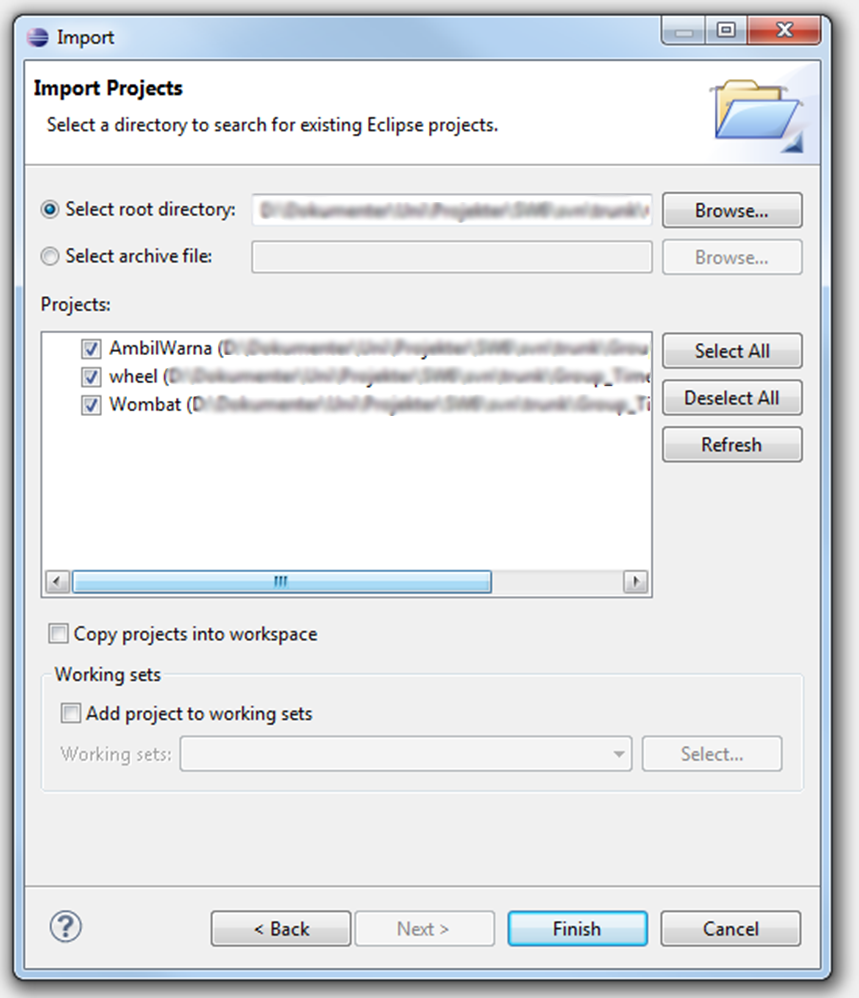
\includegraphics[scale=0.2]{Images/how_to_wombat/import1.png}
	\caption{Import Wombat, AmbilWarna, and wheel.}
	\label{fig:import1}
\end{figure}

Right click the Wombat project in Eclipse and click "Properties".\\
Under the "Android" pane, ensure that AmbilWarna and wheel are added as project libraries, figure \ref{fig:add_libs}.

\begin{figure}[H]
	\centering
		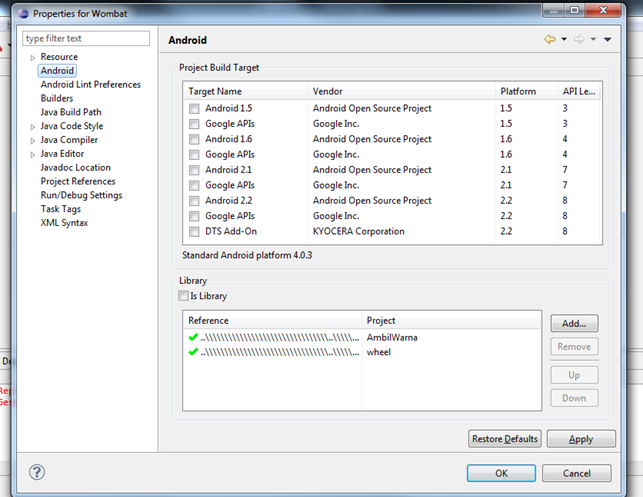
\includegraphics[scale=0.5]{Images/how_to_wombat/add_libs.png}
	\caption{Add AmbilWarna and wheel as project libraries.}
	\label{fig:add_libs}
\end{figure}

In case Eclipse fails to recognize the libraries in the libs folder, manually add the three JAR files in Wombat/libs on svn as external JARs, in Wombat - Properties, figure \ref{fig:external_jar}.

\begin{figure}[H]
	\centering
		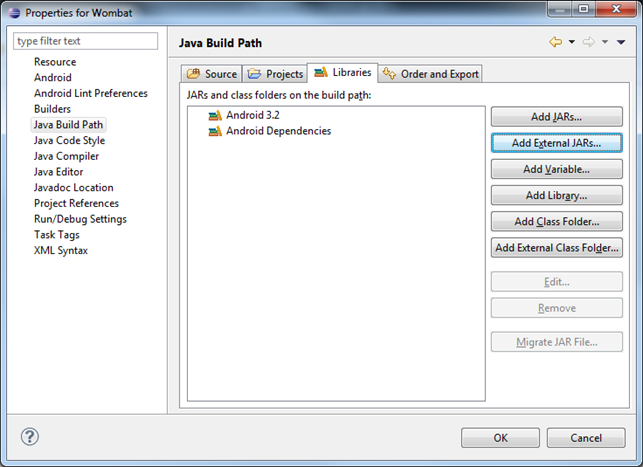
\includegraphics[scale=0.5]{Images/how_to_wombat/external_jar.png}
	\caption{Add Oasis, \texttt{TimerLib}, and \texttt{DrawLib} as external JARs if Eclipse cant recognize them in the libs folder.}
	\label{fig:external_jar}
\end{figure}

\subsection*{Extras}
To edit the \texttt{TimerLib} and \texttt{DrawLib} the two projects has to be imported to the workspace in Eclipse, figure \ref{fig:import2}.

\begin{figure}[H]
	\centering
		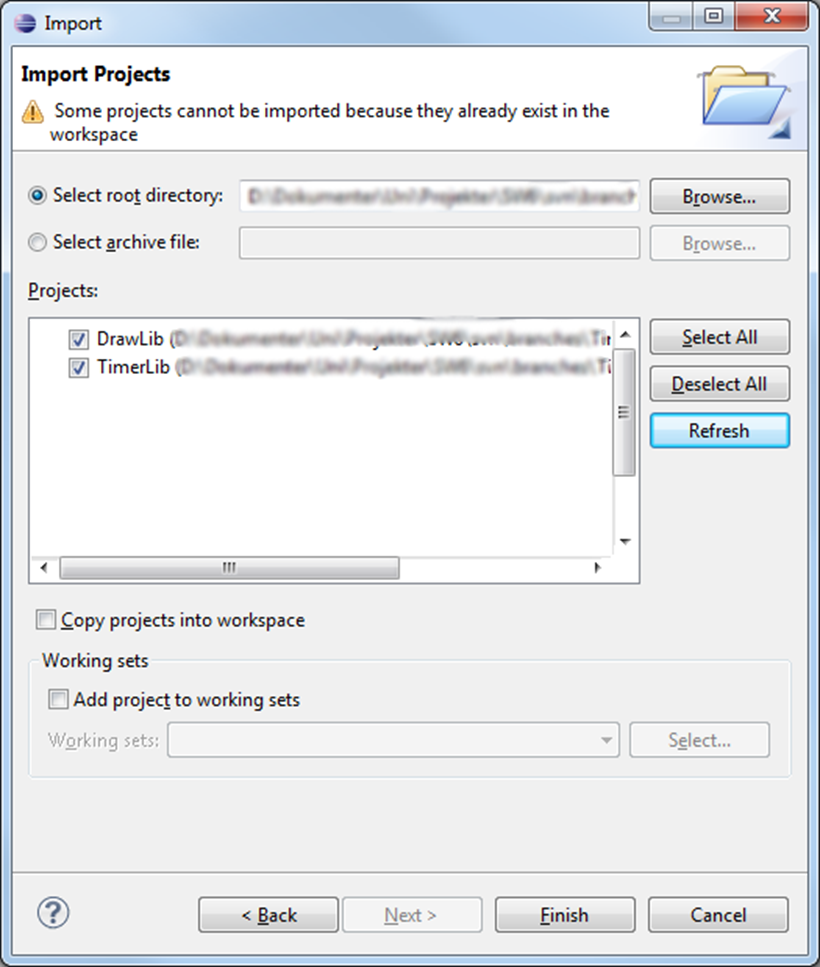
\includegraphics[scale=0.22]{Images/how_to_wombat/import2.png}
	\caption{Import TimerLib and DrawLib to the workspace.}
	\label{fig:import2}
\end{figure}

To debug the \texttt{TimerLib} and \texttt{DrawLib} in WOMBAT the projects has to be added as libraries in the Wombat properties, with AmbilWarna and wheel, figure \ref{fig:add_timer_draw_lib}.
Then the \texttt{TimerLib} and \texttt{DrawLib} JARs has to be deleted from the libs folder or the Java Build Path library, to avoid a compile error.

\begin{figure}[H]
	\centering
		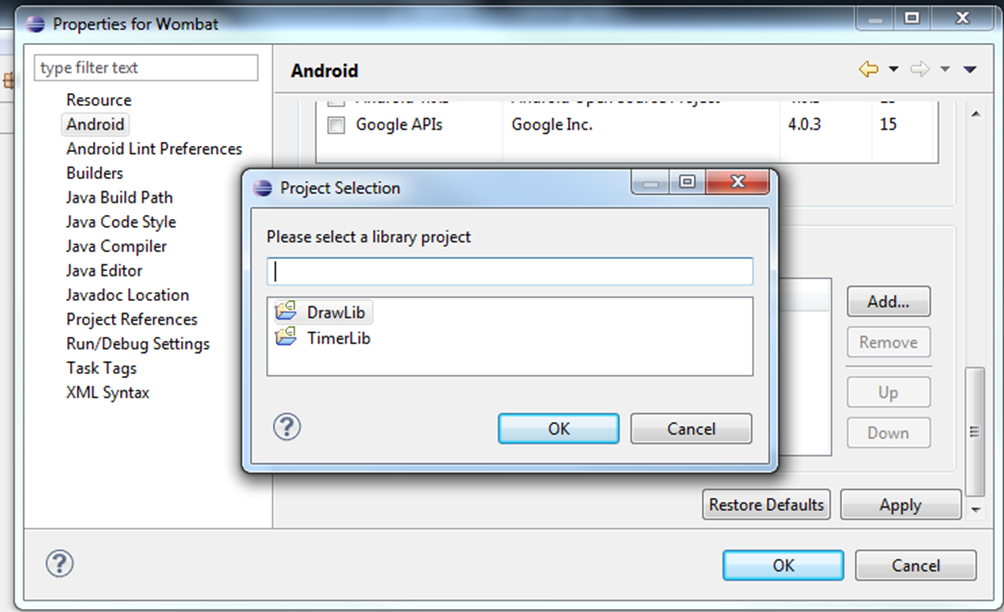
\includegraphics[scale=0.2]{Images/how_to_wombat/add_timer_draw_lib.png}
	\caption{Add \texttt{TimerLib} and \texttt{DrawLib} as project libraries.}
	\label{fig:add_timer_draw_lib}
\end{figure}

\clearpage
\section{GIRAF Installation for Android 3.2 Tablet}
\begin{enumerate}
	\item Find the "How to install" folder
	\item Connect the device to the computer
	\item	Move the two folders Pictogram and GIRAF to the root of the device
	\item	Disconnect the device from the computer.
	\item On the device open the file explorer - e.g. "Mine fil." application
	\item	On the device navigate to the "GIRAF Installer" folder and install the APK file
  \item Click "Installer" and accept all five applications
	\item On the device open OasisApp to insert Test Data - With "Tilføj Test Data"
\end{enumerate}